%% bare_conf.tex
%% V1.4b
%% 2015/08/26
%% by Michael Shell
%% See:
%% http://www.michaelshell.org/
%% for current contact information.
%%
%% This is a skeleton file demonstrating the use of IEEEtran.cls
%% (requires IEEEtran.cls version 1.8b or later) with an IEEE
%% conference paper.
%%
%% Support sites:
%% http://www.michaelshell.org/tex/ieeetran/
%% http://www.ctan.org/pkg/ieeetran
%% and
%% http://www.ieee.org/

%%*************************************************************************
%% Legal Notice:
%% This code is offered as-is without any warranty either expressed or
%% implied; without even the implied warranty of MERCHANTABILITY or
%% FITNESS FOR A PARTICULAR PURPOSE!
%% User assumes all risk.
%% In no event shall the IEEE or any contributor to this code be liable for
%% any damages or losses, including, but not limited to, incidental,
%% consequential, or any other damages, resulting from the use or misuse
%% of any information contained here.
%%
%% All comments are the opinions of their respective authors and are not
%% necessarily endorsed by the IEEE.
%%
%% This work is distributed under the LaTeX Project Public License (LPPL)
%% ( http://www.latex-project.org/ ) version 1.3, and may be freely used,
%% distributed and modified. A copy of the LPPL, version 1.3, is included
%% in the base LaTeX documentation of all distributions of LaTeX released
%% 2003/12/01 or later.
%% Retain all contribution notices and credits.
%% ** Modified files should be clearly indicated as such, including  **
%% ** renaming them and changing author support contact information. **
%%*************************************************************************


% *** Authors should verify (and, if needed, correct) their LaTeX system  ***
% *** with the testflow diagnostic prior to trusting their LaTeX platform ***
% *** with production work. The IEEE's font choices and paper sizes can   ***
% *** trigger bugs that do not appear when using other class files.       ***                          ***
% The testflow support page is at:
% http://www.michaelshell.org/tex/testflow/


\documentclass[10pt, journal]{IEEEtran}
%\documentclass[10pt, journal, compsocconf]{IEEEtran}
%\documentclass[conference]{IEEEtran}
% Some Computer Society conferences also require the compsoc mode option,
% but others use the standard conference format.
%
% If IEEEtran.cls has not been installed into the LaTeX system files,
% manually specify the path to it like:
% \documentclass[conference]{../sty/IEEEtran}


\usepackage{CJK}

% Some very useful LaTeX packages include:
% (uncomment the ones you want to load)


% *** MISC UTILITY PACKAGES ***
%
%\usepackage{ifpdf}
% Heiko Oberdiek's ifpdf.sty is very useful if you need conditional
% compilation based on whether the output is pdf or dvi.
% usage:
% \ifpdf
%   % pdf code
% \else
%   % dvi code
% \fi
% The latest version of ifpdf.sty can be obtained from:
% http://www.ctan.org/pkg/ifpdf
% Also, note that IEEEtran.cls V1.7 and later provides a builtin
% \ifCLASSINFOpdf conditional that works the same way.
% When switching from latex to pdflatex and vice-versa, the compiler may
% have to be run twice to clear warning/error messages.


% *** CITATION PACKAGES ***
%
\usepackage{cite}
% cite.sty was written by Donald Arseneau
% V1.6 and later of IEEEtran pre-defines the format of the cite.sty package
% \cite{} output to follow that of the IEEE. Loading the cite package will
% result in citation numbers being automatically sorted and properly
% "compressed/ranged". e.g., [1], [9], [2], [7], [5], [6] without using
% cite.sty will become [1], [2], [5]--[7], [9] using cite.sty. cite.sty's
% \cite will automatically add leading space, if needed. Use cite.sty's
% noadjust option (cite.sty V3.8 and later) if you want to turn this off
% such as if a citation ever needs to be enclosed in parenthesis.
% cite.sty is already installed on most LaTeX systems. Be sure and use
% version 5.0 (2009-03-20) and later if using hyperref.sty.
% The latest version can be obtained at:
% http://www.ctan.org/pkg/cite
% The documentation is contained in the cite.sty file itself.


% *** GRAPHICS RELATED PACKAGES ***
%
\ifCLASSINFOpdf
   \usepackage[pdftex]{graphicx}
  % declare the path(s) where your graphic files are
  % \graphicspath{{../pdf/}{../jpeg/}}
  % and their extensions so you won't have to specify these with
  % every instance of \includegraphics
  % \DeclareGraphicsExtensions{.pdf,.jpeg,.png}
\else
  % or other class option (dvipsone, dvipdf, if not using dvips). graphicx
  % will default to the driver specified in the system graphics.cfg if no
  % driver is specified.
   \usepackage[dvips]{graphicx}
  % declare the path(s) where your graphic files are
  % \graphicspath{{../eps/}}
  % and their extensions so you won't have to specify these with
  % every instance of \includegraphics
  % \DeclareGraphicsExtensions{.eps}
\fi
% graphicx was written by David Carlisle and Sebastian Rahtz. It is
% required if you want graphics, photos, etc. graphicx.sty is already
% installed on most LaTeX systems. The latest version and documentation
% can be obtained at:
% http://www.ctan.org/pkg/graphicx
% Another good source of documentation is "Using Imported Graphics in
% LaTeX2e" by Keith Reckdahl which can be found at:
% http://www.ctan.org/pkg/epslatex
%
% latex, and pdflatex in dvi mode, support graphics in encapsulated
% postscript (.eps) format. pdflatex in pdf mode supports graphics
% in .pdf, .jpeg, .png and .mps (metapost) formats. Users should ensure
% that all non-photo figures use a vector format (.eps, .pdf, .mps) and
% not a bitmapped formats (.jpeg, .png). The IEEE frowns on bitmapped formats
% which can result in "jaggedy"/blurry rendering of lines and letters as
% well as large increases in file sizes.
%
% You can find documentation about the pdfTeX application at:
% http://www.tug.org/applications/pdftex





% *** MATH PACKAGES ***
%
\usepackage{amsmath}
% A popular package from the American Mathematical Society that provides
% many useful and powerful commands for dealing with mathematics.
%
% Note that the amsmath package sets \interdisplaylinepenalty to 10000
% thus preventing page breaks from occurring within multiline equations. Use:
%\interdisplaylinepenalty=2500
% after loading amsmath to restore such page breaks as IEEEtran.cls normally
% does. amsmath.sty is already installed on most LaTeX systems. The latest
% version and documentation can be obtained at:
% http://www.ctan.org/pkg/amsmath

\usepackage{amsthm}

\usepackage{amssymb}



% *** SPECIALIZED LIST PACKAGES ***
%
\usepackage{algorithmic}
% algorithmic.sty was written by Peter Williams and Rogerio Brito.
% This package provides an algorithmic environment fo describing algorithms.
% You can use the algorithmic environment in-text or within a figure
% environment to provide for a floating algorithm. Do NOT use the algorithm
% floating environment provided by algorithm.sty (by the same authors) or
% algorithm2e.sty (by Christophe Fiorio) as the IEEE does not use dedicated
% algorithm float types and packages that provide these will not provide
% correct IEEE style captions. The latest version and documentation of
% algorithmic.sty can be obtained at:
% http://www.ctan.org/pkg/algorithms
% Also of interest may be the (relatively newer and more customizable)
% algorithmicx.sty package by Szasz Janos:
% http://www.ctan.org/pkg/algorithmicx

\usepackage[linesnumbered,lined,ruled]{algorithm2e}


% *** ALIGNMENT PACKAGES ***
%
\usepackage{array}
% Frank Mittelbach's and David Carlisle's array.sty patches and improves
% the standard LaTeX2e array and tabular environments to provide better
% appearance and additional user controls. As the default LaTeX2e table
% generation code is lacking to the point of almost being broken with
% respect to the quality of the end results, all users are strongly
% advised to use an enhanced (at the very least that provided by array.sty)
% set of table tools. array.sty is already installed on most systems. The
% latest version and documentation can be obtained at:
% http://www.ctan.org/pkg/array


% IEEEtran contains the IEEEeqnarray family of commands that can be used to
% generate multiline equations as well as matrices, tables, etc., of high
% quality.




% *** SUBFIGURE PACKAGES ***
\ifCLASSOPTIONcompsoc
  \usepackage[caption=false,font=normalsize,labelfont=sf,textfont=sf]{subfig}
\else
  \usepackage[caption=false,font=footnotesize]{subfig}
\fi
% subfig.sty, written by Steven Douglas Cochran, is the modern replacement
% for subfigure.sty, the latter of which is no longer maintained and is
% incompatible with some LaTeX packages including fixltx2e. However,
% subfig.sty requires and automatically loads Axel Sommerfeldt's caption.sty
% which will override IEEEtran.cls' handling of captions and this will result
% in non-IEEE style figure/table captions. To prevent this problem, be sure
% and invoke subfig.sty's "caption=false" package option (available since
% subfig.sty version 1.3, 2005/06/28) as this is will preserve IEEEtran.cls
% handling of captions.
% Note that the Computer Society format requires a larger sans serif font
% than the serif footnote size font used in traditional IEEE formatting
% and thus the need to invoke different subfig.sty package options depending
% on whether compsoc mode has been enabled.
%
% The latest version and documentation of subfig.sty can be obtained at:
% http://www.ctan.org/pkg/subfig




% *** FLOAT PACKAGES ***
%
%\usepackage{fixltx2e}
% fixltx2e, the successor to the earlier fix2col.sty, was written by
% Frank Mittelbach and David Carlisle. This package corrects a few problems
% in the LaTeX2e kernel, the most notable of which is that in current
% LaTeX2e releases, the ordering of single and double column floats is not
% guaranteed to be preserved. Thus, an unpatched LaTeX2e can allow a
% single column figure to be placed prior to an earlier double column
% figure.
% Be aware that LaTeX2e kernels dated 2015 and later have fixltx2e.sty's
% corrections already built into the system in which case a warning will
% be issued if an attempt is made to load fixltx2e.sty as it is no longer
% needed.
% The latest version and documentation can be found at:
% http://www.ctan.org/pkg/fixltx2e


%\usepackage{stfloats}
% stfloats.sty was written by Sigitas Tolusis. This package gives LaTeX2e
% the ability to do double column floats at the bottom of the page as well
% as the top. (e.g., "\begin{figure*}[!b]" is not normally possible in
% LaTeX2e). It also provides a command:
%\fnbelowfloat
% to enable the placement of footnotes below bottom floats (the standard
% LaTeX2e kernel puts them above bottom floats). This is an invasive package
% which rewrites many portions of the LaTeX2e float routines. It may not work
% with other packages that modify the LaTeX2e float routines. The latest
% version and documentation can be obtained at:
% http://www.ctan.org/pkg/stfloats
% Do not use the stfloats baselinefloat ability as the IEEE does not allow
% \baselineskip to stretch. Authors submitting work to the IEEE should note
% that the IEEE rarely uses double column equations and that authors should try
% to avoid such use. Do not be tempted to use the cuted.sty or midfloat.sty
% packages (also by Sigitas Tolusis) as the IEEE does not format its papers in
% such ways.
% Do not attempt to use stfloats with fixltx2e as they are incompatible.
% Instead, use Morten Hogholm'a dblfloatfix which combines the features
% of both fixltx2e and stfloats:
%
% \usepackage{dblfloatfix}
% The latest version can be found at:
% http://www.ctan.org/pkg/dblfloatfix




% *** PDF, URL AND HYPERLINK PACKAGES ***
%
\usepackage{url}
% url.sty was written by Donald Arseneau. It provides better support for
% handling and breaking URLs. url.sty is already installed on most LaTeX
% systems. The latest version and documentation can be obtained at:
% http://www.ctan.org/pkg/url
% Basically, \url{my_url_here}.




% *** Do not adjust lengths that control margins, column widths, etc. ***
% *** Do not use packages that alter fonts (such as pslatex).         ***
% There should be no need to do such things with IEEEtran.cls V1.6 and later.
% (Unless specifically asked to do so by the journal or conference you plan
% to submit to, of course. )

\usepackage{bm}
\usepackage{multirow}
\usepackage{booktabs}
\usepackage{tabu}
\usepackage{colortbl}
\usepackage[table*]{xcolor}
\usepackage{rotating}
\usepackage{sidecap}
\definecolor{tabcolor}{rgb}{.132,.133,.135}  
\xdefinecolor{gray95}{gray}{0.65}
\xdefinecolor{gray25}{gray}{0.8}
\newcommand{\tabincell}[2]{\begin{tabular}{@{}#1@{}}#2\end{tabular}}
\makeatletter
\newcommand{\thickhline}{%
    \noalign {\ifnum 0=`}\fi \hrule height 1pt
    \futurelet \reserved@a \@xhline
}
\newcolumntype{"}{@{\hskip\tabcolsep\vrule width 1pt\hskip\tabcolsep}}
\makeatother

% correct bad hyphenation here
\hyphenation{op-tical net-works semi-conduc-tor}

\newtheorem{definition}{Definition}
\newtheorem{theorem}{Theorem}
\newtheorem{corollary}{Corollary}
\newtheorem{lemma}{Lemma}
\DeclareGraphicsRule{.png}{eps}{.bb}{}

\begin{document}
% paper title
% Titles are generally capitalized except for words such as a, an, and, as,
% at, but, by, for, in, nor, of, on, or, the, to and up, which are usually
% not capitalized unless they are the first or last word of the title.
% Linebreaks \\ can be used within to get better formatting as desired.
% Do not put math or special symbols in the title.
\title{A Hybrid-based Conical Area Evolutionary Algorithm for Community Detection from Signed Social Networks}


\author{
\IEEEauthorblockN{Weiqin~Ying\IEEEauthorrefmark{1},~\IEEEmembership{Member,~IEEE}, Pengfei Chao\IEEEauthorrefmark{1}, Yuehong~Xie\IEEEauthorrefmark{1}, Zhenyu~Wang\IEEEauthorrefmark{1}, Yu Wu\IEEEauthorrefmark{2}}

\IEEEauthorblockA{\IEEEauthorrefmark{1}School of Software Engineering, South China University of Technology, Guangzhou 510006, China}

\IEEEauthorblockA{\IEEEauthorrefmark{2}School of Computer Science and Educational Software, Guangzhou University, Guangzhou 510006, China}

\thanks{Corresponding author: Y. Wu (wuyu@gzhu.edu.cn)}
\thanks{
			This work was supported in part by the Natural Science Foundation of Guangdong Province, China, under Grant 2015A030313204,
			in part by the Pearl River S\&T Nova Program of Guangzhou under Grant 2014J2200052,
			in part by the National Natural Science Foundation of China under Grant 61203310 and Grant 61503087,
			in part by the Fundamental Research Funds for the Central Universities, SCUT, under Grant 2017MS043,
            in part by the Guangdong Province Science and Technology Project under Grant 2015B010131003 and
            in part by the China Scholarship Council (CSC) under Grant 201406155076 and Grant 201408440193.}

}

% conference papers do not typically use \thanks and this command
% is locked out in conference mode. If really needed, such as for
% the acknowledgment of grants, issue a \IEEEoverridecommandlockouts
% after \documentclass

% for over three affiliations, or if they all won't fit within the width
% of the page, use this alternative format:
%
%\author{\IEEEauthorblockN{Michael Shell\IEEEauthorrefmark{1},
%Homer Simpson\IEEEauthorrefmark{2},
%James Kirk\IEEEauthorrefmark{3},
%Montgomery Scott\IEEEauthorrefmark{3} and
%Eldon Tyrell\IEEEauthorrefmark{4}}
%\IEEEauthorblockA{\IEEEauthorrefmark{1}School of Electrical and Computer Engineering\\
%Georgia Institute of Technology,
%Atlanta, Georgia 30332--0250\\ Email: see http://www.michaelshell.org/contact.html}
%\IEEEauthorblockA{\IEEEauthorrefmark{2}Twentieth Century Fox, Springfield, USA\\
%Email: homer@thesimpsons.com}
%\IEEEauthorblockA{\IEEEauthorrefmark{3}Starfleet Academy, San Francisco, California 96678-2391\\
%Telephone: (800) 555--1212, Fax: (888) 555--1212}
%\IEEEauthorblockA{\IEEEauthorrefmark{4}Tyrell Inc., 123 Replicant Street, Los Angeles, California 90210--4321}}


% use for special paper notices
%\IEEEspecialpapernotice{(Invited Paper)}


% make the title area
\maketitle

% As a general rule, do not put math, special symbols or citations
% in the abstract
\begin{abstract}
Mining and analyzing community structures on social networks has drawn a great deal of attention during the past decades. Various social relationships, such as friends and foes, can be abstracted as signed social networks (SNs) containing both positive and negative links. However, most of existing community detection (CD) methods are designed primarily for unsigned networks containing only positive links. Therefore, it is significant to explore and design effective and efficient CD methods for SNs. In this paper, we first utilize decomposable characteristic of modularity Q to establish a bi-objective model for community detection in SNs. Afterwards, a conical area evolutionary algorithm based on Q-modularity (CAEAh-SN) is developed to solve this bi-objective model. Furthermore, a new tournament selection mechanism based on Q-modularity is applied to accelerate the convergence of modularity Q. Experimental results on both benchmark networks and random generated large SNs indicate that, compared with the existing algorithm MEAs-SN, CAEAh-SN not only achieves better community structures in term of both Q-modularity and NMI metrics, but also has stronger robustness to the SNs with high noises.
\end{abstract}


\begin{IEEEkeywords}
	Signed Social Networks, Community Detection, Bi-objective Optimization, Evolutionary Algorithms
\end{IEEEkeywords}
% no keywords
% For peer review papers, you can put extra information on the cover
% page as needed:
% \ifCLASSOPTIONpeerreview
% \begin{center} \bfseries EDICS Category: 3-BBND \end{center}
% \fi
%
% For peerreview papers, this IEEEtran command inserts a page break and
% creates the second title. It will be ignored for other modes.
%\IEEEpeerreviewmaketitle


\section{Introduction} \label{section:introduction}
In the real world, entities and relationships between them can be, in general, represented as various social networks (SN), such as friendship networks, Internet, neural networks and even
metabolic networks. Digging out useful data information from various networks has received considerable attention among researchers. With the deep study of social networks, it is found that the majority of social networks have the characteristics of community structures, and each of them can be divided into many communities in various sizes. In most situations, the higher connection density between nodes implies a higher possibility they lie in the same community \cite{newman2001structure,girvan2002community,radicchi2004defining,dinh2015effective}.


Specifically, a social network where there exists both positive and negative edges is called a signed social network (SNs). For instance, there are not only ``like", ``respect", ``cooperation", ``promote" on behalf of positive connections, but also ``hate", ``contempt", ``competition", ``inhibition" on behalf of negative connections in an interpersonal network. In unsigned networks, the community structure is defined as a group of nodes or vertices which have dense connections within groups and sparse connections between groups. Whereas for SNs, communities are defined not only by the density of links but also by the tendencies of links. That is to say, the links should be densely positive and sparsely negative in a community while densely negative and sparsely positive between communities. Compared with unsigned social networks, SNs reflect the real social networks more realistically \cite{wu2016partition}. In view of this consideration, methods for community detection from SNs have been the focus of many recent efforts \cite{newman2004fast,lancichinetti2008benchmark,gulikers2017spectral,pizzuti2012multiobjective,newman2016community,zhang2016community}.

In the last few decades, many classic approaches based on graph segmentation, such as betweenness centrality, minimum-cut and modularity optimization, have been proposed to uncover community structure in networks.  In these classic approaches, the formation of communities can be attributed to the ternary closure relationship and the competition of nodes \cite{felzenszwalb2004efficient,su2015quadratic}. Therefore, these classic approaches based on graph segmentation focus on identifying the strength of the edges between nodes.



 %Next, we review some classic methods and recent evolutionary algorithms successfully applied to CD.

In the betweenness centrality approach, the betweenness centrality index is essential in the analysis of social networks, but costly to compute. Motivated by the fast-growing need to compute centrality indices SNs on large, Ulrik et al. \cite{brandes2001faster} presented a faster algorithm for betweenness centrality. This  efficient algorithm is based on a new accumulation technique with a recursion formula that integrates well with traversal algorithms solving the single-source shortest-paths problem, and thus exploiting the sparsity of typical instances.

The minimum-cut graph partitioning divides the nodes to minimize the connection between the clusters and is suitable for networks where the number of partitions is known in advance and the size of each partition is similar. Based on minimum-cut graph partitioning, Shi et al. \cite{ shi2000normalized} treated image segmentation as a graph partitioning problem and further proposed a novel global criterion, the normalized cut, for solving the perceptual grouping problem in vision. This criterion measures both the total dissimilarity between the different groups as well as the total similarity within the groups, which aims at extracting the global impression of an image.

The community detection can be regarded as community prediction when the number of communities is unknown. In particular, Girvan and Newman \cite{newman2004analysis} presented the concept of modularity, one of the most known criteria for community detection, to evaluate the quality of obtained communities. The emergence of modularity makes community prediction possible. The Louvain method \cite{blondel2008fast} was propose for fast unfolding of communities in large networks by the optimization of modularity. This method includes two phases. First, each node of the network is assigned a different community. For each node, if the gain of modularity takes place by removing this node from its community and by placing it in the community of one of its neighbours, the Louvain method adds this node to the community of this neighbour. This process is repeated iteratively until no positive gain is possible. The second phase considers the communities formed in first phase as new nodes. That is, this phase builts  communities of communities. Therefore, the topological structures of networks consist in hierarchical communities.


According to the intrinsic properties, the problem of CD can be generally simulated as a multi-objective optimization problem (MOP) \cite{zhou2011multiobjective}.  Evolutionary algorithms (EAs) are popular in solving MOPs and have made some achievements on the CD \cite{li2016multi,zhang2017mixed,amelio2016evolutionary,li2015overlapping,wen2017maximal,gong2014complex,gong2012community,liu2006multiagent,liu2008moving,liu2014multiobjective}. Consequently, several CD algorithms based on EAs have been proposed during the past decade.

Pizzuti \cite{pizzuti2009multi} proposed a multiobjective genetic algorithm to uncover community structure in complex network based on the degrees of nodes. To be specific, this method optimizes two objective functions, the community score and the community fitness, which measure the quality of the division in communities of a network and the number of external links respectively. Through the use of Pareto optimality theory, a partitioning of the network is identified from a set of solutions that maximizes connections inside each community and minimizes the number of links between the communities. Moreover, it returns a set of solutions at different hierarchical levels rather than a single partitioning of the network. That is, the number of communities is determined by the optimal compromise values of the objective functions. He et \ al. \cite{He2014Evolutionary} proposed another evolutionary community detection algorithm in social networks, which guided the evolutionary process using two fitness functions defined, respectively, as the average proportion of significant connection within a community and the mean vagueness of the community boundary  between any two communities.


However, the above two CD algorithms based on EAs are only available for unsigned social networks. In recent years, Liu et al. developed
a multi-objective evolutionary algorithm based on similarity for community detection from signed social networks, referred as MEAs-SN \cite{liu2014multiobjective}. First, the original similarity is extended to the signed similarity based on the social balance theory in MEAs-SN. Then, in consideration of the natural contradiction between positive and negative links, two conflict objective functions are designed, respectively, for maximizing the sum of positive similarities within communities and maximizing the sum of negative similarities between communities. In this way, an original problem of detecting communities from SNs is modeled as a multi-objective one. Furthermore, the framework of a multi-objective evolutionary algorithm based on decomposition (MOEA/D) \cite{zhang2007moea} is adopted to solve this multi-objective problem. In their rigorous experiments, the results on both benchmark networks and large-scale synthetic networks with 1000, 5000, and 10000 nodes show the effectiveness and efficacy of MEAs-SN. However, the signed similarity between a pair of vertices is based on whether they have the common neighbors and whether both of them have the same sign of positive links with the common neighbors. As a consequence, the performance of MEAs-SN decreases seriously when the community structure is sparse or the majority of the similarities between vertexes equal to 0.

In recent years, a conical area evolutionary algorithm (CAEA) \cite{weiqin2012efficient} has been further proposed  to
enhance the runtime efficiency and population diversity of MOEA/D for bi-objective optimization by employing an efficient scheme of cone decomposition. Different from MOEA/D, CAEA not only partitions a MOP into $N$ scalar subproblems, but also assigns an exclusive decision subregion to each subproblem. In addition, each subproblem uses a conical area indicator as its scalar objective to find a local non-dominated solution within its associated decision subset.

%As a result, CAEA further improves the computational efficiency of decomposition-based MOEAs for bi-objective optimization problem.

%In recent years, a conical area evolutionary algorithm (CAEA) \cite{weiqin2012efficient} has been proposed to improve the runtime efficiency and the solution quality of MOEA/D for bi-objective optimization problems.

%jiancha
In this paper, a hybrid of signed similarity and the intrinsic weight method based on CAEA, referred to as CAEAh-SN, is further developed for CD from SNs. This approach adopts the framework of CAEA to improve the runtime efficiency and the solution quality of MEAs-SN.
%Apart from the use of CAEA, two novel objective functions are specially designed based on the decomposable characteristic of the distinguished criterion, the signed modularity Q \cite{gomez2009analysis}, in order to overcome the disadvantage of the objective functions based on similarity for CD from SNs. In addition, a modularity-based tournament selection mechanism is applied to speed up the convergence by avoiding the deviation of evolutionary vectors and eliminating the poor individuals as early as possible.

%This mechanism chooses individuals with higher modularity $Q$ scores
%
%improve the solution quality in terms of modularity Q in CAEAh-SN.

%Furthermore, four benchmark SNs consisting of two illustrated SNs and two real SNs, are used to evaluate the performances of CAEAh-SN in our experiments. Afterwards, a random generator of SNs \cite{gomez2009analysis} with parameters is designed, which can control not only the scale of the generated SNs but also the noise level of community structures by adjusting the values of parameters. Finally, 180 SNs with normal parameters and the large-scale SNs are used to further evaluate the robustness of CAEAh-SN.

%The results show that:1) CAEAh-SN outperforms MEAs-SN on adaptation. Moreover, its solution is closer to the real solution. 2) CAEAh-SN further accelerate the convergence rate of modularity Q, which contributes to finding the optimal solution in less evolutions.

%Section \ref{section:Related work} reviews some related work on CD.

The rest of this paper is organized as follows. Section \ref{section:preliminaries} introduces the definition of CD from SNs and the strategy of conical decomposition. Section \ref{section:objectives} describes objective functions and tournament selection designed for CD from SNs. The details of CAEAh-SN are given in Section \ref{section:CAEAqSN}. Section \ref{section:experiment} discusses the experimental results and the performance comparisons. Finally, the conclusions are given in Section \ref{section:conclusion}.


%\section{Related work on CD}\label{section:Related work}

%Louvain method is scalable optimization of the Modularity can be quickly applied to large-scale network. However, a obvious shortcoming of this method is that there is a problem of identifying the limits.

%\subsection{Evolutionary Algorithm For CD}


%Although the above algorithms and measures for CD obtained a good performance in the type of networks they were target to, they were designed primarily for networks containing only positive links. The studies for SNs are much less.


\section{Preliminaries}\label{section:preliminaries}
\subsection{Community Detection from Signed Social Networks} %\label{section:preliminaries:decomposition}
A signed network $\mathbf{G}=\{V,E,w\}$. $V=\{v_1,v_2,\cdots,v_{n}\}$ is the set of nodes, $E=\{(v_i,v_j)| v_i,v_j \in V \wedge i\ne j\}$ is the set of edges,  and $w_{ij}\ne 0$ is the weight of the edge between nodes $v_i$ and $v_j$.  The weight can be larger than 0 (positive relationship) or smaller than 0 (negative relationship). If all weights are larger than 0, $\mathbf{G}$ is an unsigned network. Otherwise it is a signed network. Let $C= \{C_1,C_2,\cdots,C_{m}\}$ be a set of communities in $\mathbf{G}$, that is, $C_a \subset V $ for $k=1,2,\cdots,m$.  The problem of CD from SNs can be defined as follows:
\begin{equation}\label{equ:WEIGHT}
\begin{cases}
w_{ij}>0, & v_i \in C_l \wedge v_j \in C_l \\
w_{ij}<0, & v_i \in C_l \wedge v_j \in C_a \wedge l \neq k
\end{cases}
\end{equation}
where $l,k=1,2\cdots,m$. In other words, the problem aims to find a community structure that maximizes both the sum of positive links within communities and that of negative links between communities.

\subsection{Cone Decomposition} \label{section:preliminaries:decomposition}


%In order to partition the decision space, a utopia point and a nadir point are firstly required in the objective space. $A \subseteq \Omega$ is a set of solutions. The utopia point and the nadir point over A are defined as (\ref{eqn:POINT}).
%\begin{eqnarray}
%\label{eqn:POINT}
%&utopia\ point& F^{\vartriangle}(A) = (f{_1^{\vartriangle}},f{_2^{\vartriangle}})\nonumber\\
%&nadir\ point& F^{\triangledown}(A) = (f{_1^{\triangledown}},f{_2^{\triangledown}})\nonumber\\
%&where& f{_i^\vartriangle} =\mathop{min}\limits_{x \in A} f_i(x), i=1,2 \nonumber\\
%&& f{_i^{\triangledown}} =\mathop{max}\limits_{x \in A} f_i(x), i=1,2
%\end{eqnarray}

%For convenience, CAEA transforms an objective vector $\mathbf{y}$ to $\overline{\mathbf{y}}$ by $\overline{\mathbf{y}}= \mathbf{y}-F^{\vartriangle}(A)$. After this transformation, the utopia point is at the origin (0,0).
%
%The observation vector for any point $\overline{\mathbf{y}}= (\overline{y}_1,\overline{y}_2)$ is $\overline{V}(\overline{\mathbf{y}})= (\bar{v}_1(\bar{\mathbf{y}}),\bar{v}_2(\bar{\mathbf{y}}))$, where $\bar{v}_i(\bar{\mathbf{y}})=\frac{\bar{y}_i}{\bar{y}_1+\bar{y}_2}$, and $i=1,2.$ This definition of CAEA means that all the points would be on the line $\bar{v}_1(\bar{\mathbf{y}})+\bar{v}_2(\bar{\mathbf{y}})=1$. Given a prescribed number of divisions N, a series of uniformly distributed observation vectors $\overline{V}^{(k)}$ can be defined as $\overline{V}^{(k)}=(\frac{k}{N-1},1-\frac{k}{N-1}),k=0,1,\cdots,N-1$, called the center observation vector. As shown in Fig.\ref{fig:CEAE:subregion}, each $\overline{V}^{(k)}$ can induce a resulting conical subregion where the observation vector of any point is closer to $\overline{V}^{(k)}$ than the other vectors.

In the cone decomposition scheme of CAEA, a utopia point and a nadir point are firstly required in the objective space in order to partition the decision space. Let $A \subseteq \Omega$ be a set of solutions. The utopia point $\mathbf{f}^{\vartriangle}(A)$ and the nadir point $\mathbf{f}^{\triangledown}(A)$ over $A$ are defined as follows:
%\begin{eqnarray}
\begin{equation}\label{eqn:POINT}
\begin{aligned}
 &\mathbf{f}^{\vartriangle}(A) = (f{_1^{\vartriangle}},f{_2^{\vartriangle}}),&\\
 &\mathbf{f}^{\triangledown}(A) = (f{_1^{\triangledown}},f{_2^{\triangledown}}),& \\
where\ & f{_i^\vartriangle} =\mathop{min}\limits_{x \in A} f_i(x),& \\
 &f{_i^{\triangledown}} =\mathop{max}\limits_{x \in A} f_i(x),& i=1,2.
\end{aligned}
\end{equation}
%\end{eqnarray}

%&utopia\ point&
%
%&nadir\ point&

For convenience, CAEA transforms an objective vector $\mathbf{y}$ to $\overline{\mathbf{y}}$ by $\overline{\mathbf{y}}= \mathbf{y}-\mathbf{f}^{\vartriangle}(A)$. After this transformation, the utopia point is at the origin (0,0). The observation vector for any point $\overline{\mathbf{y}}= (\overline{y}_1,\overline{y}_2)$ is $\overline{\textbf{V}}(\overline{\mathbf{y}})= (\bar{v}_1(\bar{\mathbf{y}}),\bar{v}_2(\bar{\mathbf{y}}))$, where $\bar{v}_i(\bar{\mathbf{y}})=\frac{\bar{y}_i}{\bar{y}_1+\bar{y}_2}$, and $i=1,2$. It means that all the observation vectors are on the line $\bar{v}_1(\bar{\mathbf{y}})+\bar{v}_2(\bar{\mathbf{y}})=1$. Given a prescribed number of divisions $N$, a series of uniformly distributed observation vectors can be defined as $\overline{\textbf{V}}^{(k)}=(\frac{k}{N-1},1-\frac{k}{N-1}),k=0,1,\cdots,N-1$, called the center observation vector, which induces a resulting conical subregion $C^{(k)}$ where the observation vector of any point is closer to $\overline{\textbf{V}}^{(k)}$ than to the other center vectors.

In CAEA, each sub-problem aims to search a local optimal solution with the minimal conical area in its associated conical sub-region.
Given a solution $\overline{\mathbf{y}}{'}\in {C}^{(k)}, 0\leq k\leq N-1$,
the conical area for $\overline{\mathbf{y}}{'}$ in ${C}^{(k)}$ is the area of the
portion $\tilde{C}(\overline{\mathbf{y}}{'})= \{\overline{\mathbf{y}}\in
{C}^{(k)}|\neg(\overline{\mathbf{y}}{'}\prec \overline{\mathbf{y}})\wedge
\overline{\mathbf{y}}\prec \overline{\mathbf{y}}^{r}\}$, written as
$s_k(\overline{\mathbf{y}}{'})$,
where $\overline{\mathbf{y}}^{r}$ is the reference point, which should be an
approximate infinity point dominated by all feasible solutions.
The \emph{k-th} conical sub-problem $g^{cone,k}(\textbf{x})$ associated with an exclusive decision sub-set $\Omega^{(k)}$ can be thereby described in the following form:
\begin{equation}
\begin{aligned}
minimize \quad &g^{cone,k}(\textbf{x})=s_k(\mathbf{f}(\textbf{x})-\mathbf{f}^{\vartriangle}(\Omega)),&\\
subject\ to \quad  &\textbf{x}\in\Omega^{(k)}.&
\end{aligned}
\end{equation}

 %If , cone area $OU^{(2)}{\overline{y}}'L^{(1)}$ is defined as follows:

To be specific, it is inferred by further derivation that if $\overline{\mathbf{y}}' \in C^{(k)}$, $1\leq k \leq N-2$, the conical area for $\overline{\mathbf{y}}'$ can be efficiently calculated as follows:
\begin{equation}
s_k(\overline{\mathbf{y}}')= 0.5 \frac{1}{a}{\overline{y}_{1}'}^2 +0.5 b{\overline{y}_{2}'}^2 -\overline{y}_{1}'\overline{y}_{2}',
\end{equation}
where $a=\frac{k-0.5}{N-k-0.5}$ and $b=\frac{k+0.5}{N-k-1.5}$.
Otherwise, if $\overline{\mathbf{y}}' \in C^{(0)}$, $s_0(\overline{\mathbf{y}}')= 0.5 b{\overline{y}_{2}'}^2 +(\overline{y}_{2}^r-\overline{y}_{2}')\overline{y}_{1}'$ can be reached. Similarly, it can be obtained that $s_{N{-}1}(\overline{\mathbf{y}}')= 0.5 \frac{1}{a}{\overline{y}_{1}'}^2 + (\overline{y}_{1}^r-\overline{y}_{1}')\overline{y}_{2}'$ in the case $\overline{\mathbf{y}}' \in C^{(N-1)}$.

%If ${\overline{y}}' \in C^{(k)}, 0\leq k \leq N-1$, the conical area of ${\overline{y}}'$ is defined as $S({\overline{y}}')$.

\section{similarity and weight hybrid-based Multi-objective Model}\label{section:objectives}
%\subsection{Objective Functions for CD from SNs}
This paper builds a multi-objective model based on hybrid of similarity and weight for CD from SNs. 
Instead of using weight of two adjacent nodes directly, Huang et al.  proposed structural similarity to denote the local connectivity density of any two adjacent nodes in  a unsigned weighted undirected network. 
%The similarity $s(i, j)$ for $i, j \in V $ is defined as follows:
%\begin{equation}
%S_{signed}(i,j)=\frac{\sum\limits_{x\in\Gamma(i)\cap\Gamma(j)} w(i,x)\cdot w(j,x) }
%{\sqrt{\sum\limits_{x \in \Gamma(i)} w^2(i,x)} \cdot \sqrt{\sum\limits_{x \in \Gamma(j)} w^2(j,x)}},
%\end{equation}
Based on the social balance theory, Liu et al. designed a signed similarity to make it applicable in signed networks. Specifically, They classified the relationships between a pair of nodes $i, j$ and their mutual neighbor $x$ into three cases. Fig. \ref{fig:CAEAh-SN:case} gives the example for these three nodes' relationships. 
\begin{figure}[!htbp]
 	\centering
 	\subfloat[]{
 		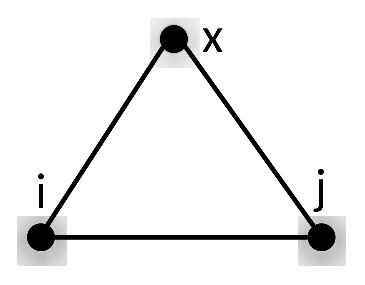
\includegraphics[width = 0.3\linewidth]{./Figure/case1.eps}
 		\label{fig:CAEAh-SN:case1}
 	}
 	\subfloat[]{
 		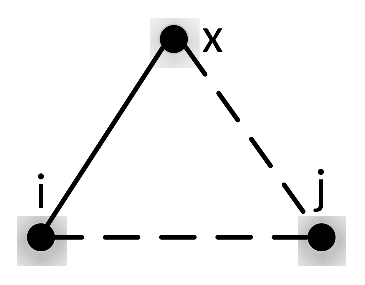
\includegraphics[width = 0.3\linewidth]{./Figure/case2.eps}
 		\label{fig:CAEAh-SN:case2}
 	} 
	\subfloat[]{
 		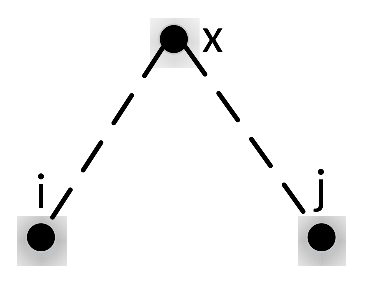
\includegraphics[width = 0.3\linewidth]{./Figure/case3.eps}
 		\label{fig:CAEAh-SN:case3}
 	} 
 	\caption{Example for three nodes' relationships. Solid lines are positive and dashed lines are negative. (a)Both i, x and j, x are friends. (b) i, x are friends and j, x are foes. (c)Both i, x and j, x are foes.}
 	\label{fig:CAEAh-SN:case}
 \end{figure}
Thus, the signed similarity is defined as
\begin{equation}
S_{signed}(i,j)=\frac{\sum\limits_{x\in\Gamma(i)\cap\Gamma(j)} \Psi(x)}
{\sqrt{\sum\limits_{x \in \Gamma(i)} w^2(i,x)} \cdot \sqrt{\sum\limits_{x \in \Gamma(j)} w^2(j,x)}},
\end{equation}
where
$$\Psi(x)=
\begin{cases}
0			  & \text{$w(i,x)  < 0 \, and \,  w(j,x) < 0$}\\
w(i,x)\cdot w(j,x) & \text{otherwise} 
\end{cases}$$
%It is worth noting that, signed similarity is based on whether a pair of nodes have a common neighbor or not and the connection properties between the pair of nodes and their neighbors. That is, the total similarity of the pair of nodes is a superposition of the number of their shared nodes and the nature of the connection. In particular, when a common neighbor is negatively connected to them, symbolic similarity treats this similarity as zero. Therefore, the performance of MEAsSN is unsatisfactory when the community structure is sparse (fewer common neighbors) or multiple pairs of nodes are negatively connected with their common neighbors.

It is worth noting that, the total signed similarity of $i, j$ is depended on the number of their common neighbors and the property of their connections. Therefore, the performance of MEAs$\_$SN turns down when detecting SNs that the community structure  is sparse  or the most of connections are negative. Given this situation, we  use the weight of this pair nodes  instead of no relationship between $i$ and $j$ in case (c). So a hybrid of signed similarity and the intrinsic weight between $i$ and $j$ to denote strength of these two adjacent nodes, is calculated as
\begin{equation}
SW(i,j)=\frac{\sum\limits_{x\in\Gamma(i)\cap\Gamma(j)} \Psi(x)}
{\sqrt{\sum\limits_{x \in \Gamma(i)} w^2(i,x)} \cdot \sqrt{\sum\limits_{x \in \Gamma(j)} w^2(j,x)}},
\end{equation}
where
$$ \Psi(x)=\left\{
\begin{array}{rcl}
|w(i,j)| \cdot w(i,j)     &      & {w(i,x)  < 0 \, and \,  w(j,x)<0}\\
w(i,x)\cdot w(j,x)      &      & {otherwise}
\end{array} \right. $$

In general, the links should be densely positive and sparsely negative in a community while densely negative and sparsely positive between communities.  In view of this consideration, a strength-based multi-objective model is designed in this paper. The model consists of the following two objective functions:
\begin{eqnarray}
\label{eqn:bi-objective function}
&minimize&   F(C)=\{f^+(C),f^-(C)\} \nonumber\\
&subject\ to&   C=(c_1,c_2,...,c_m)\in \Omega,
\end{eqnarray}
where 
%\begin{eqnarray}
%\label{eqn:bi-objective functions}
%&&   f^+(C)=\frac{1}{m}\sum\limits_{a = 0}^m \frac{P_{out}^{C_a}}{P_{in}^{C_a}+P_{out}^{C_a}} \\
%&&   f^-(C)=\frac{1}{m}\sum\limits_{a = 0}^m \frac{N_{in}^{C_a}}{N_{in}^{C_a}+N_{out}^{C_a}}
%\end{eqnarray}
%\begin{align}
%&P_{in}^{C_a}=\sum_{v_i,v_j \in C_a \wedge (v_i,v_j) \in E} max(SW(i,j), 0),\\
%&N_{in}^{C_a}=\sum_{v_i,v_j \in C_a \wedge (v_i,v_j) \in E} min(SW(i,j),0),\\
%&P_{out}^{C_a}=\sum_{v_i \in C_a \wedge v_j \in c_b \wedge a \neq b \wedge (v_i,v_j) \in E}max(SW(i,j),0), \\
%&N_{out}^{C_a}=\sum_{v_i \in C_a \wedge v_j \in c_b \wedge a \neq b \wedge (v_i,v_j) \in E} min(SW(i,j),0).
%\end{align}
\begin{eqnarray}
\label{eqn:bi-objective functions}
&&   f^+(C)=\frac{1}{m}\sum\limits_{a = 0}^m \frac{PS_{out}^{C_a}}{PS_{in}^{C_a}+PS_{out}^{C_a}} \\
&&   f^-(C)=\frac{1}{m}\sum\limits_{a = 0}^m \frac{NS_{in}^{C_a}}{NS_{in}^{C_a}+NS_{out}^{C_a}}
\end{eqnarray}
\begin{align}
&PS_{in}^{C_a}=\sum_{v_i,v_j \in C_a } max(SW(i,j), 0),
\label{PSin} \\ 
&NS_{in}^{C_a}=\sum_{v_i,v_j \in C_a } min(SW(i,j),0),  \label{NSin} \\  
&PS_{out}^{C_a}=\sum_{v_i \in C_a \wedge v_j \in C_b \wedge a \neq b }max(SW(i,j),0), \label{PSout} \\ 
&NS_{out}^{C_a}=\sum_{v_i \in C_a \wedge v_j \in C_b \wedge a \neq b } min(SW(i,j),0), 
\label{NSout}
\end{align}
%\begin{align}
%&PS_{in}^{C_a}=\sum_{v_i,v_j \in C_a \wedge (v_i,v_j) \in E} max(SW(i,j), 0),
%\label{PSin} \\ 
%&NS_{in}^{C_a}=\sum_{v_i,v_j \in C_a \wedge (v_i,v_j) \in E} min(SW(i,j),0),  \label{NSin} \\  
%&PS_{out}^{C_a}=\sum_{v_i \in C_a \wedge v_j \in c_b \wedge a \neq b \wedge (v_i,v_j) \in E}max(SW(i,j),0), \label{PSout} \\ 
%&NS_{out}^{C_a}=\sum_{v_i \in C_a \wedge v_j \in c_b \wedge a \neq b \wedge (v_i,v_j) \in E} min(SW(i,j),0). 
%\label{NSout}
%\end{align}

$(v_i,v_j) \in E$ is the set of edges, $C$ is a possible partition in the partition space $\Omega$ of network, and $C_a$ is one of communities in $C$.
$PS_{in}^{C_a}$ and $NS_{in}^{C_a}$ denote the sums of positive and negative strength, respectively, in community $C_a$, while $PS_{out}^{C_a}$ and $NS_{out}^{C_a}$ represent the sums of positive and negative strength, respectively, between $C_a$ and the other communities. $f^+(C)$ implies maximizing the tendency of forming the community structure $C$, and $f^-(C)$ denotes minimizing the tendency of destroying the community structure $C$. These two objectives are often contradict to each other and both are located in an interval [0,1].
Specifically, the strength-based multi-objective model has three major advantages for CD from SNs. 
%Foremost, since two objectives are derived from the popular modularity, it guarantees the reasonability of the model. 
Foremost, since two objectives are derived from the hybrid of signed similarity and weight, it guarantees the robustness of the model. 
Afterwards, the multi-objective model can be solved by multi-objective evolutionary algorithms which possess better mechanisms of diversity maintenance than single objective ones. In addition, the optimization of the first objective function $f^+(C)$ tends to divide a network into lager communities, while the optimization of another objective function $f^-(C)$ tends to divide a
network into small communities. Thus we can obtain a set of tradeoff solutions, which represent
the network partitions at different resolution scales.


\section{Proposed Algorithm: CAEA{\upshape h}-SN}\label{section:CAEAhSN}
\subsection{Strength-based Initializer of Chromosome}\label{section:CAEAqSN:chromosome}



\begin{figure}[!htbp]
 	\centering 
 	%\subfloat[]
	\thesubfigure
 		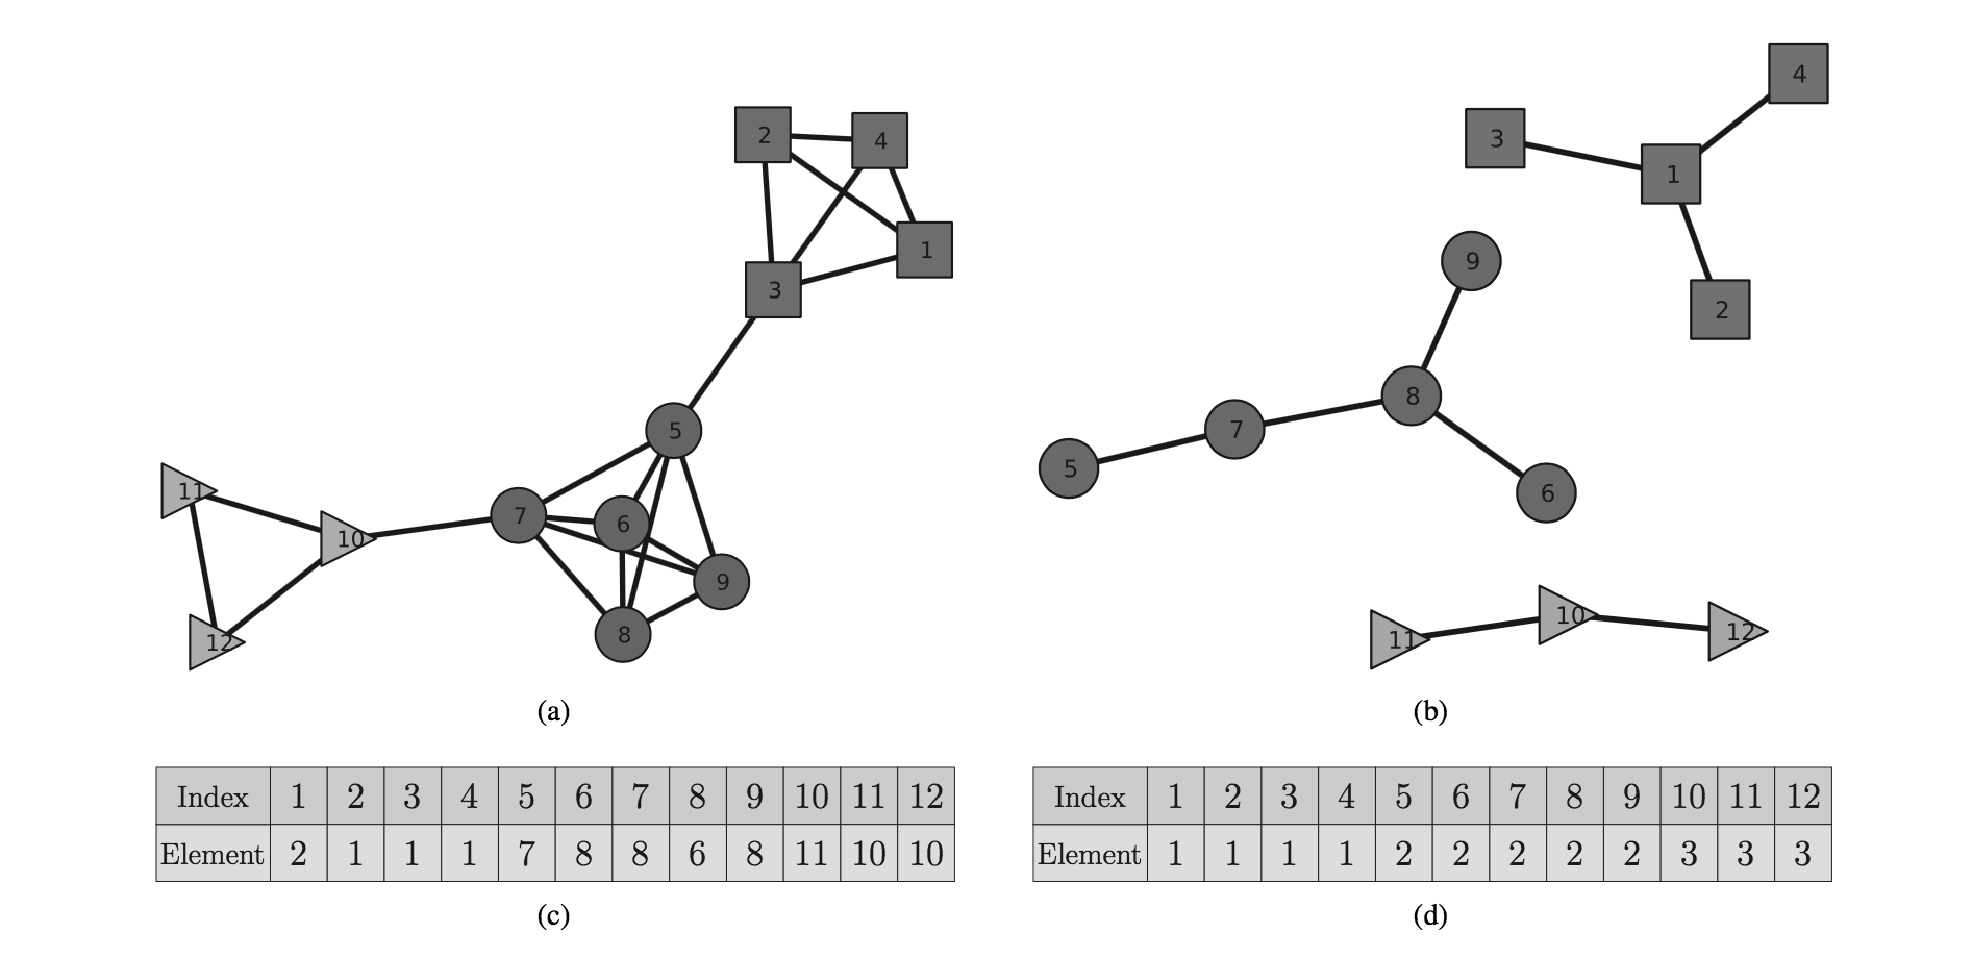
\includegraphics[width = 1.0\linewidth]{./Figure/locus-based.eps}
 	 \nonumber
 	\caption{Example for locus-based adjacency representation. Solid lines are positive and dashed lines are negative. (a) A network with 3 communitie. (b) The locus-based representation for a solution. (c)Three connected components representing the three communities. (d) The corresponding genotype of this network}
 	\label{fig:CAEAh-SN:locus-based}
 \end{figure}

%%pfchao20171008
The representation and initialization of chromosome have a major impact on the effectiveness and efficiency of EAs for CD. The proposed algorithm, CAEAh-SN, adopts a vector with $n$ elements to directly represent the community structure of an individual $\textbf{x}$:
\begin{equation}
\textbf{x}=(x_{1},x_{2},...,x_{n}),
\end{equation}
where $x_i$ denotes that node $v_i$ belongs to $C_{x_i}$, $1 \leq i \leq n$. Therefore $\textbf{x}$ is also the actual community structure. For the sake of producing a better initial population, it is necessary to design a  initializer based on the network information. The population initialization is described as follows.

%%pfchao20171008
Let $\pmb{\pi}=\{\pi_1,\pi_2,...,\pi_n\}$ be a permutation of all nodes in $V$ (i.e., a permutation of $\{1,2,...,n\}$). For an individual $\textbf{x}$ of the initial population, $\textbf{x}$ is conducted by the initializer from $\pmb{\pi}$. Then the initializer repeats this process until $N$ individuals are produced.

Huang et al. used a similarity-based quality function for any local community $C_a$, called the tightness \cite{huang2011towards}, to design the initializer. Formally, the original tightness for community $C_a$ is defined as follow:
\begin{equation}
T(C_a)=\frac{S_{in}^{C_a}}{S_{in}^{C_a}+S_{out}^{C_a}},
\end{equation}
where $S_{in}^{C_a}$ and $S_{out}^{C_a}$ mean, respectively, the internal and external similarities of community $C_a$ in an unsigned network. Liu et al. further introduced the similarity-based signed tightness \cite{liu2014multiobjective} in MEAs-SN to extend $T$ to the signed situation. The similarity-based signed tightness for community $C_a$ is labeled as
\begin{equation}\label{section:CAEAqSN:MEAsTsigned}
T_{signed}(C_a)= \frac{P_{in}^{C_a}-N_{in}^{C_a}}{P_{in}^{C_a}-N_{in}^{C_a}+P_{out}^{C_a}},
\end{equation}
%where $P_{in}^{C_a}$ and $P_{out}^{C_a}$ denote the positive internal and external similarities of community $C_a$, respectively, and $N_{in}^{C_a}$ defines the negative internal similarity of $C_a$. It is worth noting that the negative external similarity of $C_a$, referred as $N_{out}^{C_a}$, is discarded in Eq. \ref{section:CAEAqSN:MEAsTsigned}. In this paper, we propose a strength-based signed tightness, written as $T_{w}$, to make full use of four kinds of weights within a community structure in the signed situation.
where $P_{in}^{C_a}$ and $P_{out}^{C_a}$ denote the positive internal and external similarities of community $C_a$, respectively, and $N_{in}^{C_a}$ defines the negative internal similarity of $C_a$. Based on this form, we propose a strength-based signed tightness, written as $T_s$,
%It is worth noting that the negative external similarity of $C_a$, referred as $N_{out}^{C_a}$, is discarded in Eq. \ref{section:CAEAqSN:MEAsTsigned}. In this paper, we propose a strength-based signed tightness, written as $T_{w}$,
Formally, the strength-based signed tightness for community $C_a$
is calculated as follow:
\begin{equation}\label{eqn:CAEAh-SN_Ts}
T_{s}(C_a)= \frac{PS_{in}^{C_a}-NS_{in}^{C_a}}{PS_{in}^{C_a}-NS_{in}^{C_a}+PS_{out}^{C_a}},
\end{equation}
%\begin{equation}\label{eqn:CAEATsigned}
%\begin{aligned}
%T_{s}(C_a)= \frac{w^+}{w^++w^-}P_{w}^{C_a} + \frac{w^-}{w^++w^-}N_{w}^{C_a} \\
%P_{w}^{C_a}=\frac{P_{win}^{C_a}}{P_{win}^{C_a}+P_{wout}^{C_a}},\ N_{w}^{C_a}=\frac{N_{wout}^{C_a}}{N_{win}^{C_a}+N_{wout}^{C_a}}
%\end{aligned}
%\end{equation}
where $PS_{in}^{C_a}$, $NS_{in}^{C_a}$ and $PS_{out}^{C_a}$ have been introducted in Eqs. (\ref{PSin}), (\ref{NSin}) and  (\ref{PSout}), respectively. 
%represent the ratios of internal positive weights and external negative ones, respectively, for community $C_a$.  

It is worth noting that the internal positive ratio $PS_{in}^{C_a}$ and the external negative ratio $NS_{in}^{C_a}$ contribute to the total tightness proportionally to the positive and negative strengths.  As a consequence, even negative weights in signed SNs can be also naturally handled for the strength-based tightness.
In particular, a larger tightness $T_{s}(C_a)$ is obtained if $PS_{in}^{C_a}$ is far greater than $PS_{out}^{C_a}$ and $NS_{out}^{C_a}$ is far greater than $NS_{in}^{C_a}$, which means that most positive links lie inside community $C_a$ and most negative links lie outside $C_a$. Obviously, $T_{s}(C_a)$ is in the range of $[0,1]$, and a higher value of $T_{s}(C_a)$ implies a higher quality of community $C_a$.

Let $C = \{c_1, c_2, ..., c_m \}$ be a set of communities. Afterwards, for each node $v_{\pi_i}$ in $\pmb{\pi}$ in order, the initializer checks whether node $v_{\pi_i}$ can increase the tightness $T_s$ of current community $C_a$, that is, whether the following equation can be satisfied:
%%pfchao20171008
\begin{equation} \label{eqn:Tsigned}
T_{s}(C_a \cup \{v_{\pi_i}\}) > T_{s}(C_a).
\end{equation}
As long as a community is found to satisfy Eq. \ref{eqn:Tsigned}, the process terminates and this node is added to this community. Otherwise this node itself forms a new community and this new community is added to $C$. The details of the initializer are presented in Algorithm \ref{algorithm:CAEAqSN:Initializer}.
\begin{algorithm}[!htbp]
	\caption{Strength-based Initializer} \label{algorithm:CAEAqSN:Initializer}	

    \KwOut{
           $C=\{c_1,c_2,...,c_m\}$;
    }

    {$C \leftarrow \phi$; $jcomm \leftarrow null$};

    \For{$i \leftarrow 1$ \KwTo $n$}{
       \For{$k \leftarrow 1$ \KwTo $|C|$}{
          \If{$T_{s}(C_k \cup \{v_{\pi_i}\}) > T_{s}(C_k)$}{
                $C_k \leftarrow C_k \cup \{v_{\pi_i}\}$;
                update $T_{s}(C_k)$;
                $jcomm \leftarrow k$;
                break;
          }
        } 	
	}

    \If{$jcomm = null$}{
        $C \leftarrow C \cup \{v_{\pi_i}\}$;
    }

\end{algorithm}

\subsection{Evolutionary Operators}\label{section:CAEAqSN:operators}

%%pfchao20171008
We adopt the one-way crossover operator introduced in \cite{tasgin2007community}.
The one-way crossover randomly selects two parental individuals from the population, with one individual $\textbf{x}^{p1}$ set as the initial child individual $\textbf{x}^c$. Then a node is randomly selected as the crossover seed $i$. Let $find\_community(\textbf{x}^{p2}[i])$ return the nodes set (denoted as $C_{find}$) of community $\textbf{x}^{p2}[i]$. Thereafter, all the
nodes in $C_{find}$ of $\textbf{x}^{p2}$ are also assigned to the same community in the initial child individual $\textbf{x}^c$ chromosome.

Algorithm \ref{algorithm:CAEAqSN:crossover} describes the procedure of the crossover operator. It can be easily inferred from Algorithm \ref{algorithm:CAEAqSN:crossover} that the crossover operator has the time complexity of $O(n)$, which increase linearly with the size of network.

%%pfchao20171008
\begin{algorithm}[!htbp]
	\caption{Crossover operator} \label{algorithm:CAEAqSN:crossover}
	
	\KwIn{$n$: the number of network nodes;
          $\textbf{x}^{p1},\textbf{x}^{p2}$: a pair of parental individuals.
    }
    \KwOut{
           $\textbf{x}^c$:the child individual.
    }

    \For{$j\leftarrow 1$ \KwTo $n$}
	{\label{code:InitializeDirection:calcNeighbor:begin}
		
		{$\textbf{x}^c[j] \leftarrow \textbf{x}^{p1}[j] $}\;
	}\label{code:InitializeDirection:calcNeighbor:end}

    {$i\leftarrow rand() \% n $;}

    {$C_{find} \leftarrow find\_community(\textbf{x}^{p2}[i]) $;}

    \For{$v_k$ in $C_{find}$}{
        $\textbf{x}^c[k] \leftarrow \textbf{x}^{p2}[i]$; }

    {\KwRet{\rm $\textbf{x}^c$}}
\end{algorithm}



Based on signed tightness, mutation operator traverses all the neighbors of vertex $v_i$, where index $i$ is a random integer in the range $[1,n]$. If the neighbor increases the tightness of community $C$ that $v_i$ belongs to, then this neighbor is added to $C$ and the traversal terminates. The process of mutation is shown in Algorithm \ref{algorithm:CAEAqSN:crossover}, where $find\_neighbor(v_i)$ returns all neighbors of node $v_i$.

%%pfchao20171008
\begin{algorithm}[!htbp]

	\caption{Mutation operator} \label{algorithm:MOEACD:mutation}
	
	\KwIn{$n$: the number of network nodes;
          $\textbf{x}^c$: the child individual.
    }
    \KwOut{
           $\textbf{x}^c$: the child individual.
    }
    
    {$\textbf{x} \leftarrow null$;}

   \For{$i \leftarrow 1$ \KwTo $n$} {
   	{$C_{find} \leftarrow find\_community(\textbf{x}^c[i]) $}\;
   	\If{$unirand() > 0.1$ or $unirand()<T_{s}(C_{find})$} { continue;}
	\If{\rm $\textbf{x} = null$}
	{ $\textbf{x} \leftarrow \textbf{x}^c$;}
	{$j  \leftarrow  roulette\_neighbor(i)$;}
	
	{$\textbf{x}[i] \leftarrow  \textbf{x}^c[j]$;}
   }
   {$\textbf{x}^c \leftarrow \textbf{x}$;}
   
   {\KwRet{\rm $\textbf{x}^c$};}

%    {$N_{find} \leftarrow find\_neighbor(v_i)$}\;
%
%    \For{$v_k$ in $N_{find}$ }{
%        {$gene \leftarrow k$}\;
%        \If{$T_{w}(C_{find} \cup v_k) > T_{w}(C_{find})$}{
%            {$\textbf{x}^c[gene] \leftarrow \textbf{x}^c[i]$}\;
%            {$C_{find} \leftarrow C_{find} \cup v_k$}\;
%        }
%    }
 
   % {\KwRet{\rm $\textbf{x}^c$}}
\end{algorithm}
The time complexity of the mutation operator is $O(L)$, which mainly depends on the number of vertex $v_i$'s neighbors.

%\subsection{Modularity-based Tournament Selection}
%
%A tournament selection mechanism based on conical area is applied in CAEA, namely, AreaTour, which selects the individual with the larger difference between the average conical areas of its two nearest neighbors and its own conical area from two random individuals \cite{weiqin2012efficient}. Based on AreaTour, we apply $Q$ to the improved tournament selection mechanism for CD from SNs, called QmodulTour, which selects parent individuals with larger Q in order to speed up the convergence rate of the algorithm.
%In QmodulTour, firstly, we select two individuals from parent randomly. Then we calculate $Q$ by directly utilizing the values of objective functions of each individual, which can be formulated as follows:
%\begin{equation}
%Q=\frac{w^+}{w^++w^-}(1-f^+(C)) -\frac{w^-}{w^++w^-}f^-(C).
%%Q={}&\frac{2w^+}{2w^++2w^-}(1-PosQ(\textbf{x}))\\
%%{}&-\frac{2w^-}{2w^++2w^-}NegQ(\textbf{x})
%\end{equation}
%Finally, we choose the larger one and weed out the individual with poor performance as soon as possible. The procedure of QmodulTour is given in Algorithm \ref{algorithm:Tournament selectionQ}.
%It is worth noting that QmodulTour has very low computation costs since both objective values, $f^+(C)$ and $f^-(C)$, have been obtained during the objective evaluations.
%%As indicated above, compared with the AreaTour, the using of $Q$ directly instead of  difference conical areas of individuals improved efficiency significantly in QmodulTour.
%%Compared with the AreaTour(), the using of $Q_{signed}$ directly in QmodulTour() improved efficiency. Therefore, in order to further optimize the algorithm, we add the modularity $ Q_{signed} $ to parent individual selection mechanism. Calculating modularity $Q_{signed}$ of each individual, choosing the largest one When we randomly select parent individuals. Larger $ Q_{signed} $, better performance. absolutely, we can find that the measure index $ Q_{signed} $ which used in this part can be obtained by simply weighted with objectives of individuals. its formula is given below:
%
%\begin{algorithm}[!htbp]	
%	\caption{Modularity-based tournament selection} \label{algorithm:Tournament selectionQ}
%	
%	\KwOut{$k$: the index of the selected individual in the population.}
%
%	{Individuals $a$ and $b$ are first randomly selected from $\{0,1,...,N-1\}$ where $N$ denotes the population size}\;
%
%    {$Q^a \leftarrow \frac{w^+}{w^++w^-}(1-f^+(C^a)) -\frac{w^-}{w^++w^-}f^-(C^a)$}\;
%    {$Q^b \leftarrow \frac{w^+}{w^++w^-}(1-f^+(C^b)) -\frac{w^-}{w^++w^-}f^-(C^b)$}\;
%    \uIf{$ Q^a \geq Q^b$}
%    {
%        $k \leftarrow a$;
%    }\Else{
%        $k \leftarrow b$\;
%    }
%    {\KwRet{$k$};}
%%\end{algorithm}
%
%%% There is a backup of this algorithm above this line
%%\begin{algorithm}[!htbp]	
%%	\caption{Modularity-based tournament selection} \label{algorithm:Tournament selectionQ}
%%	
%%	\KwOut{ the individual with higher modularity.}
%%
%%	{Individuals $\textbf{x}^a$ and $\textbf{x}^b$ are first randomly selected from $\{0,1,...,N-1\}$ where $N$ denotes the population size}\;
%%
%%    {$Q^a \leftarrow \frac{w^+}{w^++w^-}(1-f^+(C^{\textbf{x}^a})) -\frac{w^-}{w^++w^-}f^-(C^{\textbf{x}^a})$}\;
%%    {$Q^b \leftarrow \frac{w^+}{w^++w^-}(1-f^+(C^{\textbf{x}^b})) -\frac{w^-}{w^++w^-}f^-(C^{\textbf{x}^b})$}\;
%%    \uIf{\rm $ Q^a \geq Q^b$}
%%    {
%%        \KwRet{\rm $\textbf{x}^a$};
%%    }\Else{
%%        \KwRet{\rm $\textbf{x}^b$}\;
%%    }
%
%\end{algorithm}

\subsection{Procedure of CAEAh-SN}\label{section:CAEAqSN:procedure}
It is verified that CAEA shows an excellent performance and has lower computational cost for MOPs, especially for bi-objective problems. Thus, CAEAh-SN is implemented under the framework of CAEA. It is worth noting that important concepts of CAEA have been described in Section \ref{section:preliminaries},  individual initializer and evolutionary operators are given in Section \ref{section:objectives}, and this subsection describes the pseudo-code of CAEAh-SN.
\begin{algorithm}[!htbp]
	\caption{Procedure of CAEAh-SN} \label{algorithm:CAEAh-SN}
	
	\KwIn{$\mathbf{G}=\{V,E,w\}$; $N$: the size of population;
          $Gen$: the number of generations;
    }
    \KwOut{The final population.}

    {Generate $N$ initial solutions $\textbf{C}=\{C^0,C^1,...,C^{N-1} \}$
     by Algorithm \ref{algorithm:CAEAqSN:Initializer}
    }

    \For{$i \leftarrow 1$ \KwTo $2$}{
        $f_{i}^{\vartriangle}  \leftarrow \mathop{min}\limits_{0 \leq j \leq N-1} f_i(C^j);$
        $f_{i}^{\triangledown} \leftarrow \mathop{max}\limits_{0 \leq j \leq N-1} f_i(C^j);$
    }

    {$\mathbf{f}^{\vartriangle} \leftarrow (f_{1}^{\vartriangle},f_{2}^{\vartriangle}),
     \mathbf{f}^{\triangledown} \leftarrow (f_{1}^{\triangledown},f_{2}^{\triangledown})$
    }

    {Initialize the population $P=\{\textbf{x}^0,\textbf{x}^1,...,\textbf{x}^{N-1} \}$ where $\textbf{x}^0,\textbf{x}^1,...,\textbf{x}^{N-1}=null$. Set $\textbf{C}'=\textbf{C}$.
    }

     \For{$k \leftarrow 0$ \KwTo $N-1$}{
        \If{$\textbf{C}^{(k)} \neq \phi$}{
            {$\textbf{x}^k \leftarrow \arg \mathop{min} \limits_{C \in \textbf{C}}s(\mathbf{f}(C)-\mathbf{f}^{\vartriangle})$}\;
            {$\textbf{C}' \leftarrow \textbf{C}'-\textbf{x}^k $}\;
        }
    }

    \For{$k \leftarrow 0$ \KwTo $N-1$}{
         \If{\rm $\textbf{x}^k = null$}{
            {$\textbf{x}^k \leftarrow \arg \mathop{min} \limits_{C \in \textbf{C}'}d(\overline{V}(\mathbf{f}(C)-\mathbf{f}^{\vartriangle}),\overline{V}^{(j)})$}\;
            {$\textbf{C}' \leftarrow \textbf{C}'-\textbf{x}^k $}\;
         }
    }\label{algorithm:CAEAqSN:initend}

%    {Set $nE \leftarrow N, L \leftarrow \lceil \frac{N}{10} \rceil$}
%
%    {$iL \leftarrow nE\% L$ \label{algorithm:CAEAqSN:cycle}}
%
%    \uIf{$iL < 2$}{
%        $p_1 \leftarrow iL \ast(N-1)$;
%    }\Else{
%        $p_1 \leftarrow QmodulTour()$;
%    }
%
%    {Set $p_2 \leftarrow QmodulTour()$}
   {  $p_1 \leftarrow currentGen \% N$,
      $p_2 \leftarrow rand() \% N$;}  \label{algorithm:CAEAqSN:cycle}

    {Evolution: obtain $\textbf{x}^c$ after the crossover and mutation of $\textbf{x}^{p_1},\textbf{x}^{p_2}$; Set $nE \leftarrow nE+1$;}

    {Update $\mathbf{f}^{\vartriangle},\mathbf{f}^{\triangledown}$}

    \For{$i \leftarrow 1$ \KwTo 2}{
        \If{\rm $f_i(\textbf{x}^c) < f_{i}^{\vartriangle}$}{
         {$f_{i}^{\vartriangle} \leftarrow f_i(\textbf{x}^c)$}\;
        }
        \If{\rm $f_i(\textbf{x}^c) > f_{i}^{\triangledown}$}{
         {$f_{i}^{\triangledown} \leftarrow f_i(\textbf{x}^c)$}\;
        }
    }

    {Update the solution $\textbf{x}^k$:
     $k_1$ is the index of subregion where $\textbf{x}^c$ lies and $k_2$ is the index of subregion where $\textbf{x}^{k_1}$ lies
    }

     \If{\rm $ k_1 \neq k_2 \wedge s(\textbf{f}(\textbf{x}^c)-\textbf{f}^{\vartriangle}) < s(\textbf{f}(\textbf{x}^{k_1})-\textbf{f}^{\vartriangle})$}{
         {$\textbf{x}^{k_1} \leftarrow \textbf{x}^c$}\;
     }

    {If evolution to $Gen$ generation, then stop and output the best solution, otherwise go to step \ref{algorithm:CAEAqSN:cycle} \label{algorithm:CAEAqSN:end}}

\end{algorithm}

In Algorithm \ref{algorithm:CAEAh-SN}, $\lceil \cdot \rceil$ is ceil, $d(\cdot, \cdot)$ is the Euclidean distance between two vectors, $iL$ is set to increase the selected probability of the individual in edge subregion, and $k_1$ and $k_2$ denote respectively the index of subregion where solution $c'$ and $c^{k1}$ belong to.
%%pfchao20171008
\begin{equation}
k_1 =\lfloor \frac{(N-1)(f_1(\textbf{x}^c)-f{_1^{\vartriangle}})}{f_1(\textbf{x}^c)-f{_1^{\vartriangle}}+f_2(\textbf{x}^c)-f{_2^{\vartriangle}}} +\frac{1}{2} \rfloor
\end{equation}

\begin{equation}
k_2 = \lfloor \frac{(N-1)(f_1(\textbf{x}^{k_1})-f{_1^{\vartriangle}})}{f_1(\textbf{x}^{k_1})-f{_1^{\vartriangle}}+f_2(\textbf{x}^{k_1})-f{_2^{\vartriangle}}} +\frac{1}{2} \rfloor
\end{equation}

Obviously, the first part is the initialization process from step 1 to \ref{algorithm:CAEAqSN:initend}, and the second part is evolutionary process from step \ref{algorithm:CAEAqSN:cycle} to \ref {algorithm:CAEAqSN:end}. In the evolutionary part, CAEAh-SN uses the new tournament selection mechanism (i.e., QmodulTour). QmodulTour not only accelerates the convergence rate of the modularity Q value but also simplifies the calculation since it uses the objective function of individual for comparison directly.

\section{Experiments and Analysis}\label{section:experiment}
%20170411
In this section, the performance of CAEAh-SN is evaluated on both small benchmark real SNs and large synthetic SNs, and compared with  MEAs-SN and the Louvain method. In our experiments, the population sizes of CAEAh-SN and MEAs-SN are set as $N=100$. For CAEAh-SN and MEAs-SN, the termination criterion is satisfied when the number of evolutionary generations reaches 100 on every SNs. The other parameters of MEAs-SN and the Louvain method use
the corresponding recommended values provided, respectively, by \cite{liu2014multiobjective} and \cite{blondel2008fast}. CAEAh-SN is implemented in C++, MEAs-SN is implemented in C, and a special version for SNs of Louvain method is implemented in Pajek\cite{mrvar2013pajek} 
All the three algorithms  run on an Intel Core
i5-3470 3.20 GHz PC with 4GB RAM and Windows 7 OS. To assess the overall performances of
algorithms, a total of 20 statistically independent runs of each algorithm have
been executed for each SNs.


\subsection{Performance Indicators}\label{section:experiment:indicators}
A commonly used normalized mutual information (NMI) measure  \cite{Danon2005Comparing} and the modularity, Q\cite{gomez2009analysis}, are chosen as the performance indicators in our experiments for CD from SNs. 

Based on the information theory, the NMI indicator measures the difference between the community structure obtained by an algorithm and the real structure through a confusion matrix $M$. In matrix $M$, each row represents one real community, each column denotes an obtained community, and the element $M_{ij}$ refers to the number of nodes which lie in the real community $C^{\ast}_i$ in the real structure $C^{\ast}$ and also belong to the community $C_j$ in an obtained structure $C$. Given the real structure $C^{\ast}$ and an obtained structure $C$ for a SNs, the NMI between them is defined as follows:
\begin{equation} \label{equ:NMI}
NMI(C^{\ast},C)= \frac{-2\sum_{i=1}^{m^{\ast}}\sum_{j=1}^{m}M_{ij}\log(\frac{nM_{ij}}{M_{i\cdot}M_{\cdot j}})}{\sum_{i=1}^{m^{\ast}} M_{i\cdot}\log(\frac{M_{i\cdot}}{n})+\sum_{j=1}^{m}M_{\cdot j}\log(\frac{M_{\cdot j}}{n})},
\end{equation}
where $n$ is the number of nodes, $m^{\ast}$ represents the number of the real communities in $C^{\ast}$, and $m$ indicates the number of the obtained community in $C$, $N_{i\cdot}$ and $N_{\cdot j}$ denote the sums of elements in the $i$-th row and the $j$-th column, respectively, in matrix $M$. If the obtained structures is identical to the real network structure, the value of $NMI$ takes its maximum 1. In contrast, when they are completely different, $NMI$ is equal to 0.

G$\acute{o}$mez et al.  presented a reformulation of modularity for the analysis of community structures in signed situations. Let $c_i$ denote that node $v_i$ is assigned to the community $C_{c_i}$, $w=(w_{ij})$ be the weighted adjacency matrix of a SNs where every element $w_{ij}$ represents the value of the weight in the link between node $v_i$ and $v_j$ (0 if no link exists), and $ w_{ij}^+=max\{0,w_{ij}\}$ and $w_{ij}^-=max\{0,-w_{ij}\} $ , respectively, indicate the positive and negative portions of $w_{ij}$ such that $w_{ij}=w_{ij}^+ + w_{ij}^- $. As a result, the sums of the positive and negative weights of node $v_i$ are, respectively, $ w_i^+=\sum_j w_{ij}^+ $ and $ w_i^-=\sum_j w_{ij}^- $. Furthermore, the total positive and negative weights of the SNs equal to $w^+=\sum_i w_i^+$ and $ w^-=\sum_i w_i^-$, respectively. Afterwards, the total signed modularity Q \cite{gomez2009analysis} for the SNs can be expressed in the following mathematical form:
\begin{equation}\label{Qdefinition}
\begin{aligned}
Q=\frac{1}{w^{+}+w^{-}}\sum_i\sum_j \Big[w_{ij}-(\frac{w_i^+w_j^+}{w^+}-\frac{w_i^-w_j^-}{w^-})\Big]\delta(c_i,c_j),
\end{aligned}
\end{equation}
where $\delta(c_i,c_j)$ takes the value 1 if nodes $v_i$ and $v_j$ are in the same community, i.e., $c_i=c_j$, otherwise it takes value 0. Therefore, it does not require the reference real structure. A larger value of the modularity usually indicates a better structure. In practice, the values of modularity Q for the real structures of most networks are typically in the range from 0.3 to 0.7.

%The modularity Q for a given partition is the probability of having edges falling within groups in the network minus the expected probability in an equivalent network. The edges of this equivalent network are placed at random preserving the strengths of nodes, where the strength of a node stands for the sum of the weights of its connections \cite{newman2004analysis}. In general, the larger modularity Q means that a better partition is obtained.
%
%Essentially, the total modularity Q can be decomposed into two parts as follows:
%\begin{equation}\label{Qdefinition:twoparts}
%Q=\frac{w^+}{w^++w^-}Q^+-\frac{w^-}{w^++w^-}Q^-,
%\end{equation}
%where the positive modularity $Q^+$ for the partition with only positive weights is calculated by
%\begin{equation}\label{Qdefinition:posparts}
%Q^+=\frac{1}{w^+}\sum_i\sum_j({w_{ij}}^+-\frac{{w_i}^+{w_j}^+}{w^+})\delta(c_i,c_j),
%\end{equation}
%and, similarly, the negative modularity $Q^-$ for the partition with only negative weights equals to
%\begin{equation}\label{Qdefinition:negparts}
%Q^-=\frac{1}{w^-}\sum_i\sum_j({w_{ij}}^--\frac{{w_i}^-{w_j}^-}{w^-})\delta(c_i,c_j).
%\end{equation}
%
%Eq. \ref{Qdefinition:twoparts} suggests that
%$Q^+$ and $Q^-$ contribute to the total modularity proportionally to their respective positive and negative strengths.


\subsection{Experiments on Benchmark Signed Networks} \label{section:Experiment and analysis:Benchmark}
Four benchmark signed networks, including two illustrative SNs \cite{yang2007community} with 28 nodes and two real SNs, are first detected in our experiments.
Two real SNs are the Slovene Parliamentary Party Network \cite{ferligoj1996analysis} and the Gahuku-Gama Subtribes Network  \cite{read1954cultures}. Specifically, the former describes the relationship of the 10 parties of the Slovenian Parliament in 1994, and the latter represents the political alliance and class struggle of the 16 subtribes of Gahuku-Gama.

\begin{table}[!htbp]
	\caption{The median scores of both $Q$ and NMI achieved by CAEA{\upshape h}-SN for four benchmark SNs}
	\label{table:setting:Benchmark Networks}
	\centering
	\scriptsize
	\begin{tabu} to \linewidth{X[7,c]|X[2,c]|X[2,c]}
		\toprule
		\textbf{Network} 	&	\textbf{Q}	&	\textbf{NMI}		\\
	
		\midrule
		$Illustrated$ $signed$ $network$ $\uppercase\expandafter{\romannumeral1}$	&	0.564286	&	1		\\
		\midrule
		$Illustrated$ $signed$ $network$ $\uppercase\expandafter{\romannumeral2}$	&	0.521267	&	1		\\
		\midrule
		$Slovene$ $Parliamentary$ $Party$ & 0.454733 & 1 	\\
		\midrule
		$Gahuku-Gama$ $Subtribes$ & 0.431034 & 1 	\\	
		\bottomrule
	\end{tabu}
\end{table}

 \begin{figure}[!htbp]
 	\centering
% 	\subfloat[]{
%        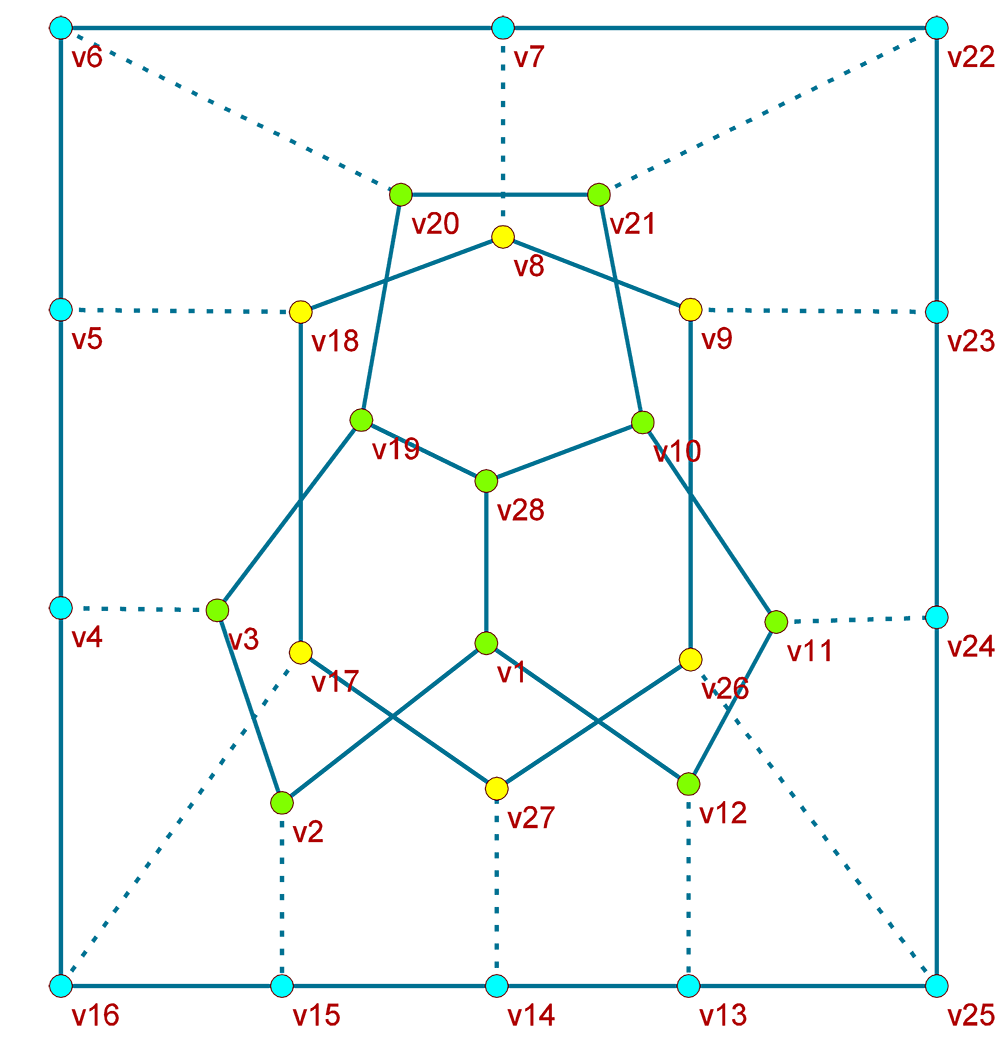
\includegraphics[width = 0.45\linewidth]{./Figure/illustrative1.png}
% 		\label{fig:CAEAh-SN:illustrative:1}
% 	}
% 	\subfloat[]{
%         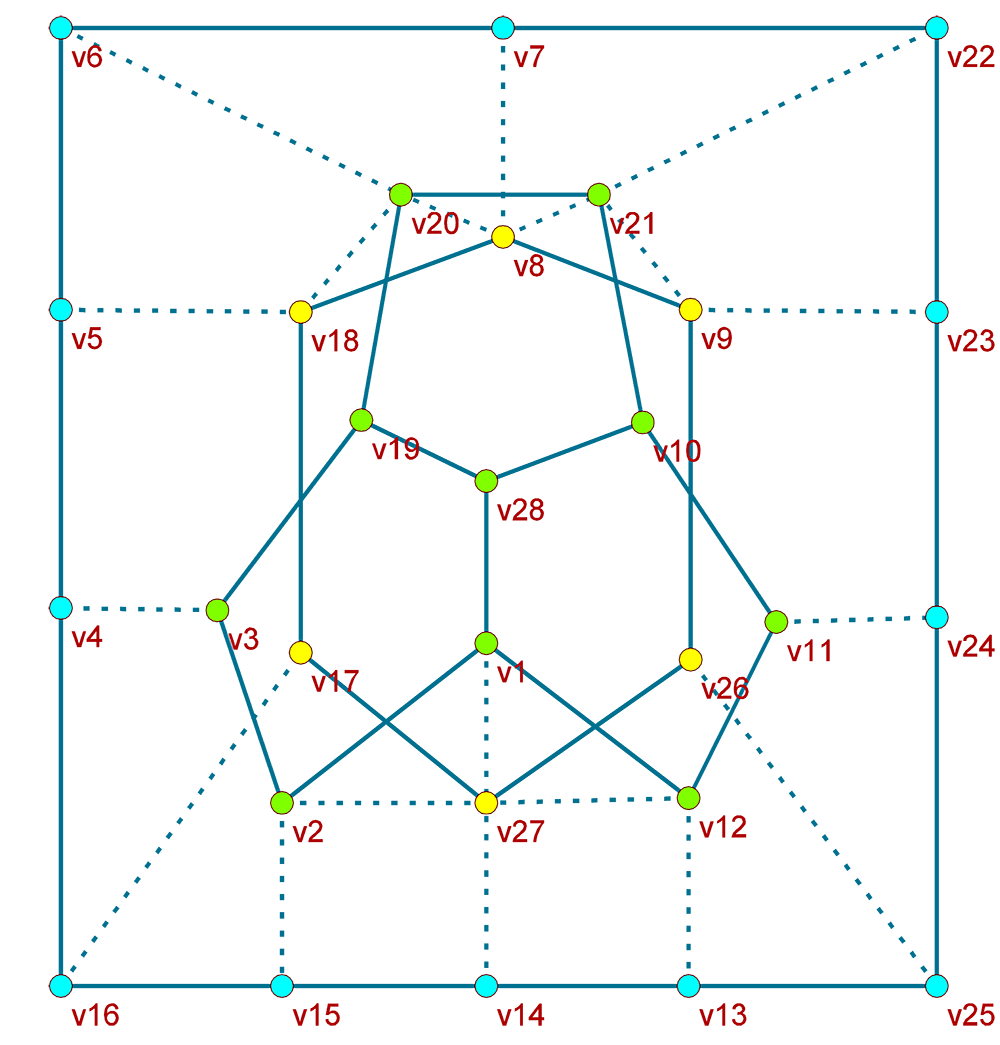
\includegraphics[width = 0.45\linewidth]{./Figure/illustrative2.png}
% 		\label{fig:CAEAh-SN:illustrative:2}
% 	}
 	\caption{Community structures with the median NMI scores obtained by CAEAh-SN for two illustrative SNs. (a) Illustrated signed network I. (b) Illustrated signed network II.}
 	\label{fig:CAEAh-SN:illustrative}
 \end{figure}


%Fig.\ref{fig:CAEAh-SN:real} shows the best partition results of two real SNs obtained by CAEAh-SN.




 \begin{figure}[!htbp]
	\centering
% 	\subfloat[]{
% 		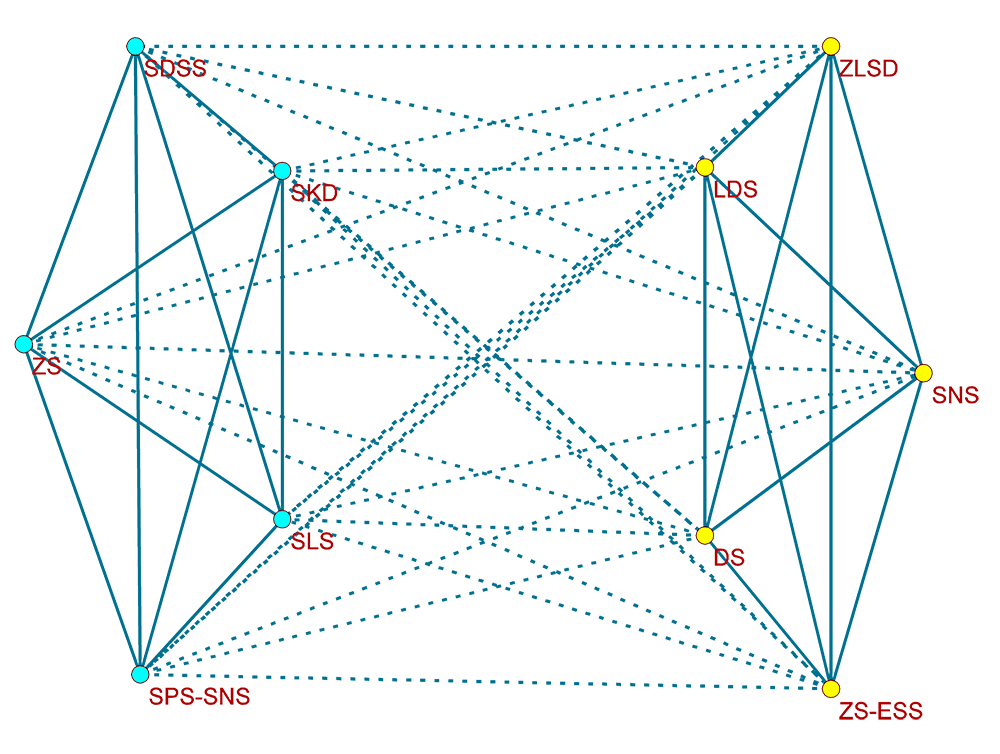
\includegraphics[width = 0.45\linewidth]{./Figure/real1.png}
% 		\label{fig:CAEAh-SN:real:1}
% 	}
% 	\subfloat[]{
% 		
\includegraphics[width = 0.45\linewidth]{./Figure/real2.png}
% 		\label{fig:CAEAh-SN:real:2}
% 	}
 	\caption{Community structures with the median NMI scores obtained by CAEAh-SN for two real SNs. (a) Slovene Parliamentary Party Network. (b) Gahuku-Gama Subtribes Network.}
 	\label{fig:CAEAh-SN:real}
 \end{figure}




Table \ref{table:setting:Benchmark Networks} records the median scores of both $Q$ and NMI achieved by CAEAh-SN for four benchmark SNs.
Afterwards, Fig. \ref{fig:CAEAh-SN:illustrative} and \ref{fig:CAEAh-SN:real} plot the community structures with the median NMI scores obtained by CAEAh-SN, respectively, for two illustrative SNs and two real SNs where solid lines denote positive links and dashed lines indicate negative links.
It can be observed from Fig. \ref{fig:CAEAh-SN:illustrative} and \ref{fig:CAEAh-SN:real} that the Illustrated signed network I and II and the Gahuku-Gama Subtribes Network are divided into three communities and the Slovene Parliamentary Party Network is into two communities, which are perfectly consistent with the numbers of communities in the real partitions of four networks.
Furthermore, Table \ref{table:setting:Benchmark Networks} indicates that the achieved NMI scores reach 1 for all these four SNs and the obtained $Q$ scores are in an expected normal range from 0.43 to 0.56. It implies that the partitions detected by CAEAh-SN are absolutely the same as the real community structures of four networks.

 %The element C-num in table \ref{table:setting:Benchmark Networks} denotes the number of communities in SNs.

%and partitions are much clear after the detection by CAEAh-SN
% the proposed algorithm CAEAh-SN is compared  on indicators NMI and Q.

\subsection{Experiments on Synthetic Signed Networks}\label{section:experiment:synthetic}
\subsubsection{SNs Generator}\label{section:experiment:synthetic:generator}
%One popular generator to generate networks with community structures is the
In order to systematically test the performance of CAEAh-SN on larger SNs, a popular SRN generator proposed in \cite{yang2007community} is used to generate larger synthetic SNs with the given community structures in our experiments. This SNs generator combines the Lancichinetti-Fortunato-Radicchi (LFR) benchmark with the generator proposed in \cite{yang2007community} and is formulated as $SRN(n,K,maxK,\tau_1,\tau_2,minc,maxc,\mu,P^+,P^-)$.
Among the above input parameters, $n$ is the total number of nodes in the SNs, $K$ and $maxK$ denotes the mean and maximum of degrees of nodes in the network, $\tau_1$ and $\tau_2$ are the respective exponential distribution coefficients of degree and community size, and $minc$ and $maxc$ indicate the smallest and largest sizes of communities. In addition, $\mu$ is the fraction of edges across communities for each node, whose increase will reduce the cohesiveness of communities.
Furthermore, $P^+$ and $P^-$ denotes the proportions of positive connections across communities and negative connections within communities, respectively.
In general, the higher value of each of $\mu$, $P^+$ and $P^-$ will result in the greater ambiguity of the community structure, thereby a larger difficulty in detecting the correct community structure.


%20170411
\subsubsection{Experiments on Synthetic SNs with Low Noise}\label{section:experiment:synthetic:results}
%20170411
In our experiments, three synthetic networks with different sizes, referred to as SRN1000, SRN5000, and SN10000, are first generated by the following parameters:
\begin{eqnarray}\label{eqn:generation 4size networks}
&&SRN(1000,20,50,2,1,20,50,0.1,0,0),  \\
&&SRN(5000,20,50,2,1,40,100,0.1,0,0),  \\
&&SRN(10000,20,50,2,1,40,100,0.1,0,0).
\end{eqnarray}
Figure \ref{fig:CAEAh-SN:SN} presents the topological structures plotted by the Pajek for four synthetic SNs where the number of edges are 1046, 5272, 34190, and 68736, respectively, for these four SNs.
Note that all four synthetic networks are in low noise levels since they are generated through the very small values of the last three parameters, i.e., $\mu=0.1$, $P^+=0$, and $P^-=0$.
\begin{figure}[!htbp]
 	\centering
% 	\subfloat[]{
% 		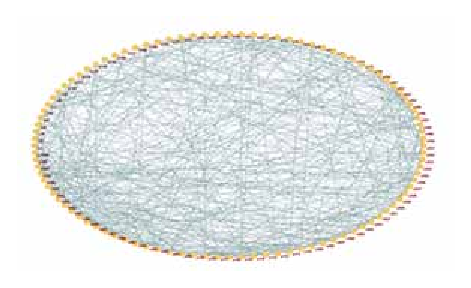
\includegraphics[width = 0.45\linewidth]{./Figure/SN100.eps}
% 		\label{fig:CAEAh-SN:SN100}
% 	}
% 	\subfloat[]{
% 		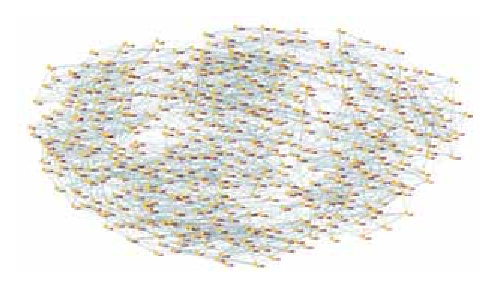
\includegraphics[width = 0.45\linewidth]{./Figure/SN500.eps}
% 		\label{fig:CAEAh-SN:SN500}
% 	} \\
% 	\subfloat[]{
% 		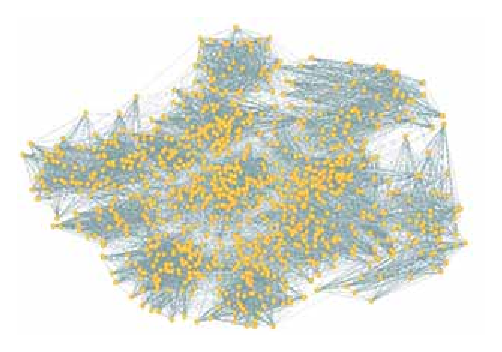
\includegraphics[width = 0.45\linewidth]{./Figure/SN1000.eps}
% 		\label{fig:CAEAh-SN:SN1000}
% 	}
% 	\subfloat[]{
% 		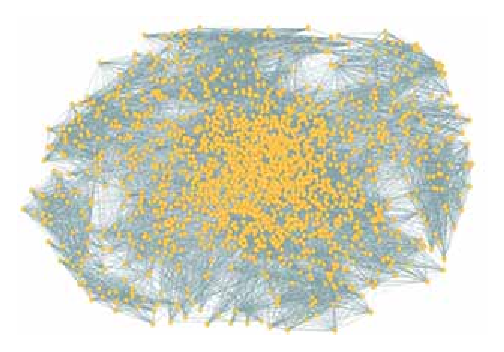
\includegraphics[width = 0.45\linewidth]{./Figure/SN2000.eps}
% 		\label{fig:CAEAh-SN:SN2000}
% 	}
 	\caption{Topological structures of four synthetic SNs.(a) SN100. (b) SN500. (c) SN1000. (d) SN2000.}
 	\label{fig:CAEAh-SN:SN}
 \end{figure}

The community structures with the median NMI scores detected by CAEAh-SN for four synthetic SNs are plotted by the Pajek in Fig. \ref{fig:CAEAh-SN:SNfinish} where
each color represents a community.

It can be seen that community structures are much clear after the detection. Four SNs are divided into 3, 17, 24 and 52 communities respectively and most of positive links are distributed in communities, and negative links are distributed between communities.
\begin{figure}[!htbp]
 	\centering
% 	\subfloat[]{
% 		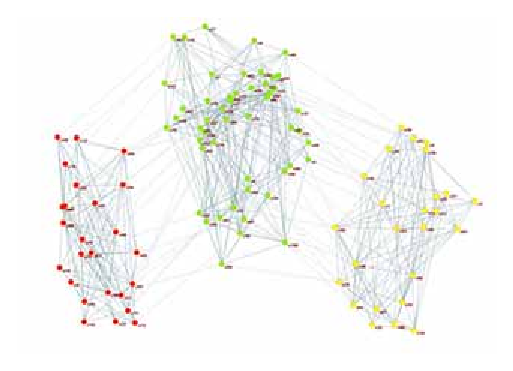
\includegraphics[width = 0.45\linewidth]{./Figure/SN100finish.eps}
% 		\label{fig:CAEAh-SN:SN100finish}
% 	}
% 	\subfloat[]{
% 		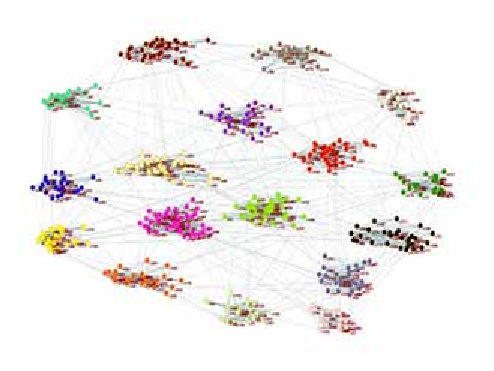
\includegraphics[width = 0.45\linewidth]{./Figure/SN500finish.eps}
% 		\label{fig:CAEAh-SN:SN500finish}
% 	} \\
% 	\subfloat[]{
% 		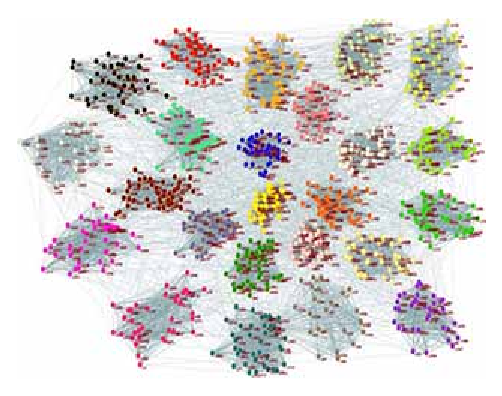
\includegraphics[width = 0.45\linewidth]{./Figure/SN1000finish.eps}
% 		\label{fig:CAEAh-SN:SN1000finish}
% 	}
% 	\subfloat[]{
% 		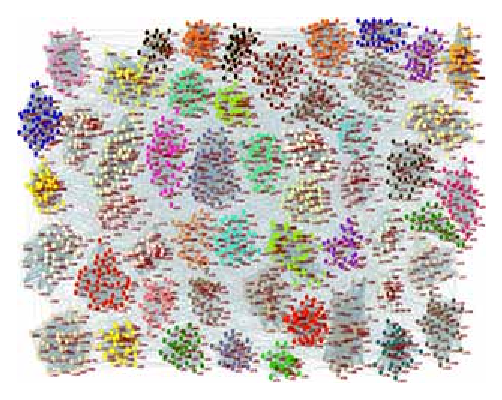
\includegraphics[width = 0.45\linewidth]{./Figure/SN2000finish.eps}
% 		\label{fig:CAEAh-SN:SN2000finish}
% 	}
 	\caption{Partitions of four synthetic SNs obtained by CAEAh-SN. Solid lines are positive and dashed lines are negative.(a)SN100. (b)SN500. (c)SN1000. (d)SN2000.}
 	\label{fig:CAEAh-SN:SNfinish}
 \end{figure}

At first, we discuss the results of the CAEAh-SN and MEAs-SN on these four synthetic SNs. In practice, value of Q for such networks typically is in the range from 0.3 to 0.7 and higher values are rare \cite{newman2004finding}. Fig. \ref{fig:CAEAh-SN:4SNmu01pp0pn0QandNMI} gives the comparison between CAEAh-SN and MEAs-SN on Q values and NMI.It is evident from Fig. \ref{fig:CAEAh-SN:4SNmu01pp0pn0QandNMI} that CAEAh-SN obtains higher Q values than MEAs-SN for all synthetic SNs, which suggests that CAEAh-SN achieves batter partitions than MEAs-SN. The Q obtained by CAEAh-SN of SN1000 and SN2000 are greater than 0.8 and the Q of network SN100 and SN500 are more than 0.5. It is clear that the performance of CAEAh-SN is batter than MEAs-SN. In the comparison of NMI values, CAEAh-SN is also superior to MEAs-SN.
\begin{figure} [!htbp]
 	\centering
% 	\subfloat[]{
% 		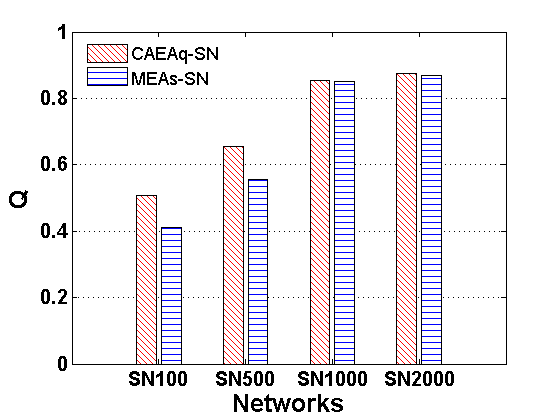
\includegraphics[width = 0.47\linewidth]{./Figure/4SNmu01pp0pn0Q.png}
% 		\label{fig:CAEAh-SN:4SNmu01pp0pn0Q}
% 	}
% 	\subfloat[]{
% 		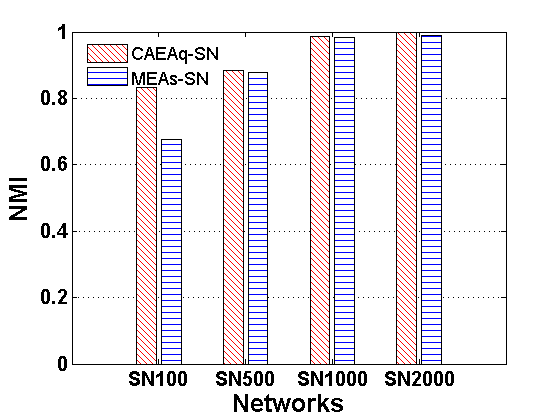
\includegraphics[width = 0.47\linewidth]{./Figure/4SNmu01pp0pn0NMI.png}
% 		\label{fig:CAEAh-SN:4SNmu01pp0pn0NMI}
% 	}
 	\caption{Comparison between CAEAh-SN and MEAs-SN on four synthetic SNs. (a)Q. (b)NMI.}
 	\label{fig:CAEAh-SN:4SNmu01pp0pn0QandNMI}
 \end{figure}

%%pfchao20171015
Table \ref{section:experiment:synthetic:results:ComputationalTime} shows the average CPU time in seconds spend by two algorithms for each test problem. As it turns out, the time taken by two algorithms increases quickly when the network size becomes larger. Table \ref{section:experiment:synthetic:results:ComputationalTime} clearly indicates that the
computational time of CAEAh-SN is always less than that of MEAs-SN when $n$ increases from 1000 to 10000.

\begin{table}[!htbp]
	\caption{Computational Time of CAEA{\upshape h}-SN and MEA{\upshape s}-SN}
    \label{section:experiment:synthetic:results:ComputationalTime}
	\centering
	\scriptsize
	\begin{tabu} to \linewidth{X[2,c]|X[1,c]|X[1,c]|X[1,c]}
		\toprule[1.05pt]
		\textbf{Algorithm} 	&	\textbf{SN1000}	&	\textbf{SN5000}	&	\textbf{SN10000} 	\\
		\midrule[1.05pt]
		$CAEAh-SN$ 	&0.5832 &18.6738 &85.6885	\\
		\midrule
		$MEAs-SN$ 	&4.7379 &72.0092 &193.4043  \\
		\bottomrule[1.05pt]
	\end{tabu}
\end{table}


\subsubsection{Experiments on Synthetic SNs with High Noise}\label{section:experiment:synthetic:Dynamicresults}


%In our experiments, three groups of synthetic networks are first generated by the following parameters:
%\begin{eqnarray}\label{eqn:generation 3 networks}
%&&SRN(1000,20,50,2,1,20,50,\mu,P^+,P^-),  \\
%&&SRN(5000,20,50,2,1,40,50,\mu,P^+,P^-), \\
%&&SRN(10000,20,50,2,1,40,100,\mu,P^+,P^-).
%\end{eqnarray}
%Note that, 90 combinations of three parameters, $\mu$, $P^+$, and $P^-$, are applied to systematically validate the robustness of CAEAh-SN
%to  noises. To be specific, $\mu$, $P^+$, and $P^-$ take values, respectively, from $\{0.1,0.3,0.5\}$, $\{0.0,0.2,0.4,0.6,0.8,1.0\}$, and $\{0.0,0.2,0.4,0.6,0.8\}$.

In our experiments, a group of synthetic networks are first generated by the following parameters:
\begin{equation}\label{eqn:SRN1000}
SN(1000,20,50,2,1,20,50,\mu,P^+,P^-) 
\end{equation}
Note that, 90 combinations of three parameters, $\mu$, $P^+$, and $P^-$, are applied to systematically validate the robustness of CAEAh-SN
to  noises. To be specific, $\mu$, $P^+$, and $P^-$ take values, respectively, from $\{0.1,0.3,0.5\}$, $\{0.0,0.2,0.4,0.6,0.8,1.0\}$, and $\{0.0,0.2,0.4,0.6,0.8\}$.


In order to evaluate the performance of CAEAh-SN systematically, we change the value of $\mu$, $P^+$, and $P^-$ to destroy SN100 and SN500. $P^+$ is in the range of $[0.0,1.0]$, $P^-$ is [0.0 0.8], $\mu$ is in the range of $[0.1,0.5]$ and they are all in the step of 0.2. For each combination of these three parameters, 30 independent runs of CAEAh-SN and MEAs-SN are conducted, and the averaged Q is reported in Figs. \ref{fig:SN100Comparison} and \ref{fig:SN500Comparison}.

\begin{table*}[!htbp]
\small
\renewcommand\arraystretch{1.4}
\centering
\caption{ the  comparison  results of NMI of  three  algorithms on  SN1000  networks}
\label{NMISN1000}
\arrayrulecolor{gray}
\begin{tabular}{|c|c|l|c|c|c|c|c|c|}\doublerulesepcolor{gray}

\thickhline
\multicolumn{3}{|c|}{$\bm{Parameters}$}      & \multicolumn{6}{c|}{$\bm{P^+}$}   \\ \thickhline
$\bm{\mu}$                   & $\bm{P^-}$    & \multicolumn{1}{c|}{$\bm{Algorithm}$} & \textbf{0.0}      & \textbf{0.2}      & \textbf{0.4}      & \textbf{0.6}      & \textbf{0.8}      & \textbf{1.0}      \\ \thickhline

\multirow{3}{*}{\textbf{0.1}} & \multirow{3}{*}{\textbf{0.0}} & CAEAh-SN & 0.991114          & 0.994233          & 0.987117          & 0.989815          & 0.991579          & 0.993818          \\ \cline{3-9}
                              &                               & MEAs-SN & 0.971001          & 0.944494          & 0.975134          & 0.955544          & 0.969295          & 0.968892          \\ \cline{3-9}
                              &                               & Louvain  & \textbf{1}        & \textbf{1}        & \textbf{1}        & \textbf{1}        & \textbf{1}        & \textbf{1}        \\ \thickhline
\multirow{3}{*}{\textbf{0.1}} & \multirow{3}{*}{\textbf{0.2}} & CAEAh-SN & \textbf{0.963302} & \textbf{0.959600}   & \textbf{0.959524} & \textbf{0.954450}  & \textbf{0.970490}  & \textbf{0.959076} \\ \cline{3-9}
                              &                               & MEAs-SN & 0.950464          & 0.942959          & 0.949074          & 0.939577          & 0.941886          & 0.946633          \\ \cline{3-9}
                              &                               & Louvain  & 0.882081          & 0.834460           & 0.771962          & 0.643372          & 0.533471          & 0.422818          \\ \thickhline
\multirow{3}{*}{\textbf{0.1}} & \multirow{3}{*}{\textbf{0.4}} & CAEAh-SN & \textbf{0.982295} & \textbf{0.979831} & \textbf{0.974207} & \textbf{0.972996} & \textbf{0.979924} & \textbf{0.984062} \\ \cline{3-9}
                              &                               & MEAs-SN & 0.758618          & 0.783190           & 0.765030           & 0.763224          & 0.743427          & 0.733261          \\ \cline{3-9}
                              &                               & Louvain  & 0.837580           & 0.716590           & 0.619024          & 0.532111          & 0.411566          & 0.260161          \\ \thickhline
\multirow{3}{*}{\textbf{0.1}} & \multirow{3}{*}{\textbf{0.6}} & CAEAh-SN & \textbf{0.985829} & \textbf{0.984057} & \textbf{0.990403} & \textbf{0.987543} & \textbf{0.989358} & \textbf{0.986422} \\ \cline{3-9}
                              &                               & MEAs-SN & 0.814883          & 0.823792          & 0.754369          & 0.718447          & 0.670672          & 0.609954          \\ \cline{3-9}
                              &                               & Louvain  & 0.806120           & 0.567816          & 0.446409          & 0.325257          & 0.236715          & 0.137532          \\ \thickhline
\multirow{3}{*}{\textbf{0.1}} & \multirow{3}{*}{\textbf{0.8}} & CAEAh-SN & 0.840622          & 0.864914          & \textbf{0.853220}  & \textbf{0.862451} & \textbf{0.853750}  & \textbf{0.845105} \\ \cline{3-9}
                              &                               & MEAs-SN & \textbf{0.873774} & \textbf{0.865268} & 0.826151          & 0.781367          & 0.737088          & 0.719427          \\ \cline{3-9}
                              &                               & Louvain  & 0.739021          & 0.533837          & 0.339940           & 0.205034          & 0.158304          & 0.113824          \\ \thickhline
\multirow{3}{*}{\textbf{0.3}} & \multirow{3}{*}{\textbf{0.0}} & CAEAh-SN & 0.971497          & 0.956623          & 0.964652          & 0.961201          & 0.963699          & 0.970149          \\ \cline{3-9}
                              &                               & MEAs-SN & 0.979256          & 0.904717          & 0.933336          & 0.962014          & 0.915149          & 0.918842          \\ \cline{3-9}
                              &                               & Louvain  & \textbf{1}        & \textbf{1}        & \textbf{1}        & \textbf{0.994774} & \textbf{0.966240}  & \textbf{0.982148} \\ \thickhline
\multirow{3}{*}{\textbf{0.3}} & \multirow{3}{*}{\textbf{0.2}} & CAEAh-SN & 0.890920           & 0.875444          & \textbf{0.916736} & 0.912256          & \textbf{0.928410}  & \textbf{0.912521} \\ \cline{3-9}
                              &                               & MEAs-SN & 0.894593          & 0.889660           & 0.908407          & \textbf{0.917575} & 0.894546          & 0.906661          \\ \cline{3-9}
                              &                               & Louvain  & \textbf{0.971276} & \textbf{0.926507} & 0.863408          & 0.699961          & 0.426157          & 0.123345          \\ \thickhline
\multirow{3}{*}{\textbf{0.3}} & \multirow{3}{*}{\textbf{0.4}} & CAEAh-SN & \textbf{0.933084} & \textbf{0.924302} & \textbf{0.921779} & \textbf{0.922807} & \textbf{0.912561} & \textbf{0.923177} \\ \cline{3-9}
                              &                               & MEAs-SN & 0.633303          & 0.657864          & 0.659809          & 0.679410          & 0.728945          & 0.775453          \\ \cline{3-9}
                              &                               & Louvain  & 0.831889          & 0.770093          & 0.603767          & 0.398792          & 0.197796          & 0.076608         \\ \thickhline
\multirow{3}{*}{\textbf{0.3}} & \multirow{3}{*}{\textbf{0.6}} & CAEAh-SN & \textbf{0.938855} & \textbf{0.912575} & \textbf{0.923704} & \textbf{0.939762} & \textbf{0.926758} & \textbf{0.943550}  \\ \cline{3-9}
                              &                               & MEAs-SN & 0.652345          & 0.629666          & 0.584359          & 0.577576          & 0.599031          & 0.659067          \\ \cline{3-9}
                              &                               & Louvain  & 0.780352          & 0.553986          & 0.311570           & 0.174698          & 0.108710           & 0.052787         \\ \thickhline
\multirow{3}{*}{\textbf{0.3}} & \multirow{3}{*}{\textbf{0.8}} & CAEAh-SN & 0.704138          & \textbf{0.687552} & \textbf{0.714041} & \textbf{0.752901} & \textbf{0.751024} & \textbf{0.717609} \\ \cline{3-9}
                              &                               & MEAs-SN & \textbf{0.774194} & 0.681446          & 0.580598          & 0.521343          & 0.598653          & 0.636236          \\ \cline{3-9}
                              &                               & Louvain  & 0.740240           & 0.380090           & 0.171606          & 0.125529          & 0.087198         & 0.074037         \\ \thickhline
\multirow{3}{*}{\textbf{0.5}} & \multirow{3}{*}{\textbf{0.0}} & CAEAh-SN & 0.914627          & 0.915391          & 0.919352          & 0.887540           & 0.889974          & 0.906223          \\ \cline{3-9}
                              &                               & MEAs-SN & 0.864806          & 0.900087          & 0.915137          & 0.895802          & 0.889345          & 0.844126          \\ \cline{3-9}
                              &                               & Louvain  & \textbf{1}        & \textbf{1}        & \textbf{1}        & \textbf{1}        & \textbf{0.985132} & \textbf{0.989914} \\ \thickhline
\multirow{3}{*}{\textbf{0.5}} & \multirow{3}{*}{\textbf{0.2}} & CAEAh-SN & 0.745901          & 0.729494          & 0.741702          & 0.738369          & 0.759910           & 0.759521          \\ \cline{3-9}
                              &                               & MEAs-SN & 0.791783          & 0.795920           & 0.783898          & \textbf{0.788930}  & \textbf{0.772516} & \textbf{0.766636} \\ \cline{3-9}
                              &                               & Louvain  & \textbf{0.993928} & \textbf{0.982256} & \textbf{0.932168} & 0.705027          & 0.263902          & 0.009384        \\ \thickhline
\multirow{3}{*}{\textbf{0.5}} & \multirow{3}{*}{\textbf{0.4}} & CAEAh-SN & 0.794617          & 0.796439          & \textbf{0.786368} & \textbf{0.794242} & \textbf{0.779132} & \textbf{0.806895} \\ \cline{3-9}
                              &                               & MEAs-SN & 0.690155          & 0.694694          & 0.694957          & 0.691602          & 0.725536          & 0.760993          \\ \cline{3-9}
                              &                               & Louvain  & \textbf{0.911017} & \textbf{0.802321} & 0.535053          & 0.325710          & 0.103395          & 0.026297         \\ \thickhline
\multirow{3}{*}{\textbf{0.5}} & \multirow{3}{*}{\textbf{0.6}} & CAEAh-SN & \textbf{0.767368} & \textbf{0.796543} & \textbf{0.808819} & \textbf{0.825660}  & \textbf{0.841407} & \textbf{0.804394} \\ \cline{3-9}
                              &                               & MEAs-SN & 0.662859          & 0.626340           & 0.574299          & 0.589592          & 0.640577          & 0.639253          \\ \cline{3-9}
                              &                               & Louvain  & 0.767311          & 0.479374          & 0.244850           & 0.137148          & 0.095462        & 0.028386        \\ \thickhline
\multirow{3}{*}{\textbf{0.5}} & \multirow{3}{*}{\textbf{0.8}} & CAEAh-SN & 0.544676          & \textbf{0.573281} & \textbf{0.668767} & \textbf{0.701072} & \textbf{0.697983} & \textbf{0.689796} \\ \cline{3-9}
                              &                               & MEAs-SN & 0.701814          & 0.505738          & 0.487485          & 0.479673          & 0.469466          & 0.475954          \\ \cline{3-9}
                              &                               & Louvain  & \textbf{0.711435} & 0.300863          & 0.170825          & 0.106195          & 0.059554         & 0.035665         \\ \thickhline
\end{tabular}
\end{table*}

%On the whole, the Q of CAEAh-SN and MEAs-SN reduce gradually with the increase of $\mu$, which implies a network with a lower density is more difficult to detect. For different combinations of $\mu$, $P^+$ and $P^-$, CAEAh-SN still works better on these networks than MEAs-SN. For example, for SN100 and SN500 when $P^->0.2$, the Q of CAEAh-SN are always higher than 0.6 and close to 0.7, while the Q of MEAs-SN is less than 0.4 when $P^+$ increases from 0 to 1.0, $P^-=0$ and $\mu =0.1$. In general, CAEAh-SN obtains obviously greater Q than MEAs for all the dynamic synthetic SNs.
\begin{table*}[!htbp]
\small
\renewcommand\arraystretch{1.4}
\centering
\caption{ the comparison results of Modularity of three algorithms on SN1000 networks}
\label{NMISN1000}
\arrayrulecolor{gray}
\begin{tabular}{|c|c|l|c|c|c|c|c|c|}\doublerulesepcolor{gray}

\thickhline
\multicolumn{3}{|c|}{$\bm{Parameters}$} & \multicolumn{6}{c|}{$\bm{P^+}$} \\ \thickhline
$\bm{\mu}$ & $\bm{P^-}$ & \multicolumn{1}{c|}{$\bm{Algorithm}$} & \textbf{0.0} & \textbf{0.2} & \textbf{0.4} & \textbf{0.6} & \textbf{0.8} & \textbf{1.0} \\ \thickhline

\multirow{3}{*}{\textbf{0.1}} & \multirow{3}{*}{\textbf{0.0}}
  & CAEAh-SN & 0.425509 & 0.426189 & 0.422164 & 0.424542 & 0.422506 & 0.421245 \\ \cline{3-9}
  & & MEAs-SN & 0.412342 & 0.417905 & 0.420392 & 0.423038 & 0.428601 & 0.388554 \\ \cline{3-9}
  & & Louvain & \textbf{0.432988} & \textbf{0.432900} & \textbf{0.432460} & \textbf{0.431458} & \textbf{0.430686} & \textbf{0.428878} \\ \thickhline
\multirow{3}{*}{\textbf{0.1}} & \multirow{3}{*}{\textbf{0.2}}
  & CAEAh-SN & 0.107424 & 0.108362 & 0.103430 & 0.101102 & 0.104087 & 0.095657 \\ \cline{3-9}
  & & MEAs-SN & 0.109136 & 0.108356 & 0.105006 & \textbf{0.107340} & \textbf{0.106764} & \textbf{0.103660}\\ \cline{3-9}
  & & Louvain & \textbf{0.114077} & \textbf{0.110016} & \textbf{0.107128} & 0.098348 & 0.095409 & 0.084879 \\ \thickhline
\multirow{3}{*}{\textbf{0.1}} & \multirow{3}{*}{\textbf{0.4}}
  & CAEAh-SN & -0.110909 & -0.111019 & -0.108502 & -0.105500 & -0.111728 & -0.113077 \\ \cline{3-9}
  & & MEAs-SN & -0.048594 & -0.052136 & -0.049868 & -0.048986 & -0.045293 & -0.041051 \\ \cline{3-9}
  & & Louvain & \textbf{0.031038} & \textbf{0.036926} & \textbf{0.042866} & \textbf{0.049581} & \textbf{0.054418} & \textbf{0.060804} \\ \thickhline
\multirow{3}{*}{\textbf{0.1}} & \multirow{3}{*}{\textbf{0.6}}
  & CAEAh-SN & -0.285827 & -0.282797 & -0.290970 & -0.289384 & -0.290531 & -0.289748 \\ \cline{3-9}
  & & MEAs-SN & -0.148397 & -0.160081 & -0.125442 & -0.120454 & -0.092117 & -0.075886 \\ \cline{3-9}
  & & Louvain & \textbf{-0.014784} & \textbf{0.006334} & \textbf{0.019578} & \textbf{0.033691} & \textbf{0.042524} & \textbf{0.049738} \\ \thickhline
\multirow{3}{*}{\textbf{0.1}} & \multirow{3}{*}{\textbf{0.8}}
  & CAEAh-SN & -0.195599 & -0.218945 & -0.211289 & -0.212345 & -0.217337 & -0.205812 \\ \cline{3-9}
  & & MEAs-SN & -0.238332 & -0.237352 & -0.225645 & -0.186293 & -0.150625 & -0.141921 \\ \cline{3-9}
  & & Louvain & \textbf{-0.021470} & \textbf{-0.001106} & \textbf{0.017053} & \textbf{0.031744} & \textbf{0.038493} & \textbf{0.042010} \\ \thickhline
\end{tabular}
\end{table*}


%20170411
On the whole, the Q of CAEAh-SN and MEAs-SN reduce gradually with the increase of $\mu$, which implies a network with a lower density is more difficult to detect. For different combinations of $\mu$, $P^+$ and $P^-$, CAEAh-SN still works better on these networks than MEAs-SN. For example, for SN100 and SN500 when $P^-=0.2$, Q of CAEAh-SN are in the vicinity of $0.2$ while Q obtained by MEAs-SN are near $0.1$ and some even are close to $0$. It is necessary to emphasize that when $P^->0.2$ the Q of MEAs-SN are almost $0$ while the most of Q obtained by CAEAh-SN are acceptable and some batter Q are more than $0.1$ for SN100 and SN500. Moreover, in some extreme case (i.e., $p^+=1.0,p^-=0.0$), CAEAh-SN obtains batter Q while MEAs-SN fails to find results whose $Q\neq 0$. In general, CAEAh-SN obtains obviously greater Q than MEAs for all the dynamic synthetic SNs.

%*****************************
\begin{figure}[!htbp]
 	\centering
 	\subfloat[]{
 		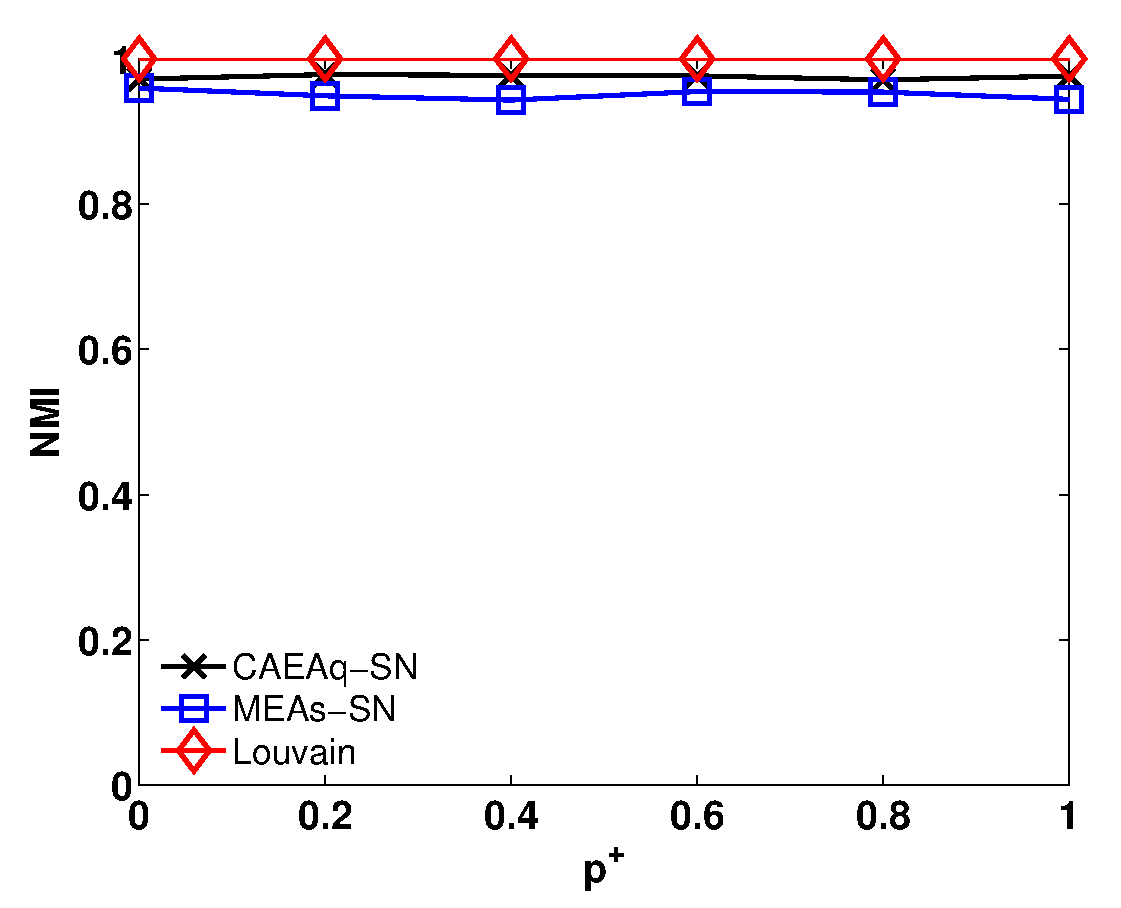
\includegraphics[width = 0.47\linewidth]{./Figure/dynamicmore/nmi5000mu01pn00.eps}	
 	}
 	\subfloat[]{
 		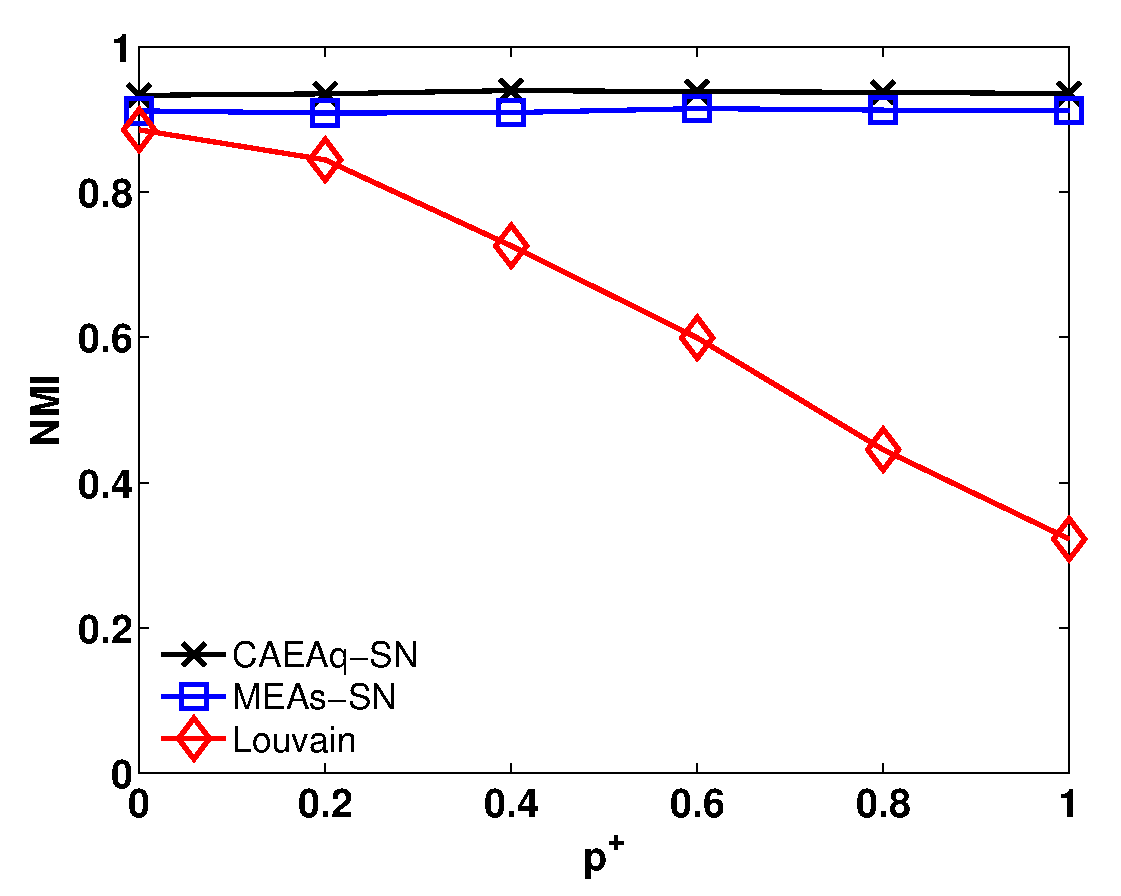
\includegraphics[width = 0.47\linewidth]{./Figure/dynamicmore/nmi5000mu01pn02.eps}	
 	}\\
 	\subfloat[]{
 		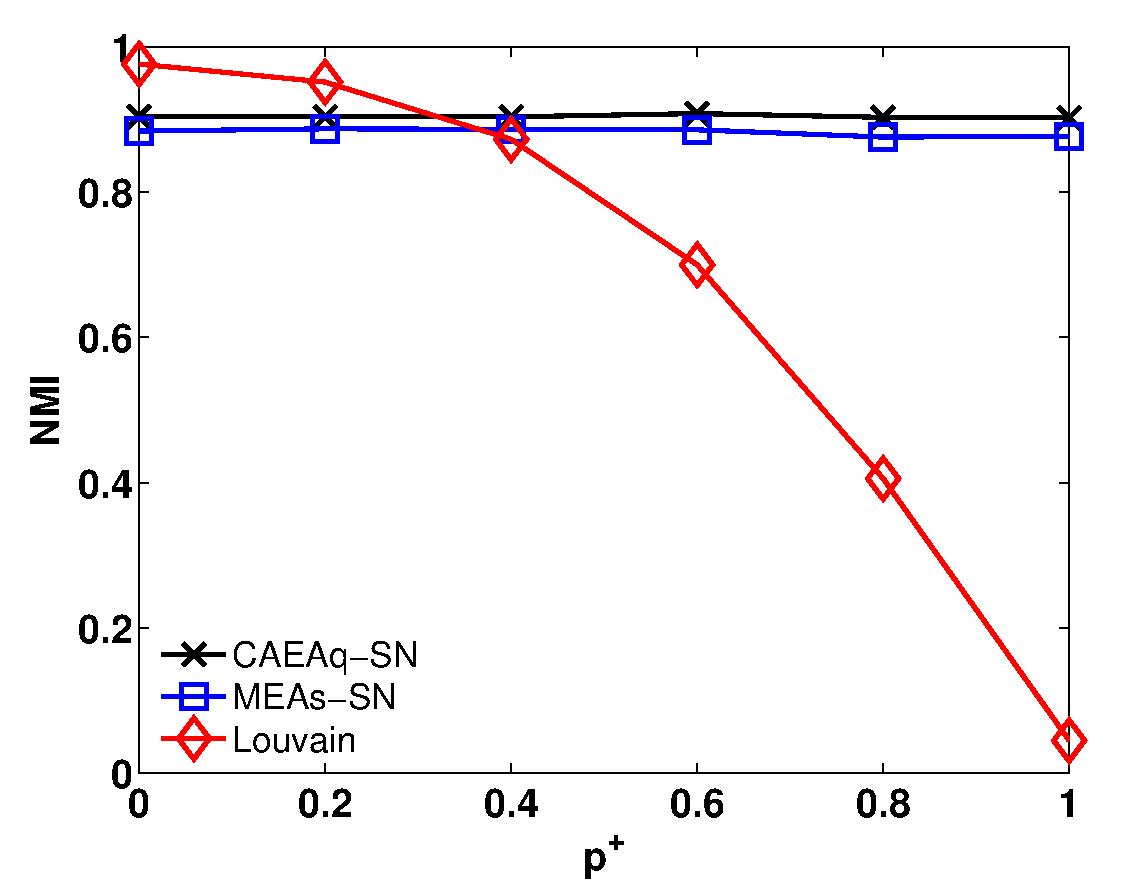
\includegraphics[width = 0.47\linewidth]{./Figure/dynamicmore/nmi5000mu03pn02.eps}	
  	}
    \subfloat[]{
 		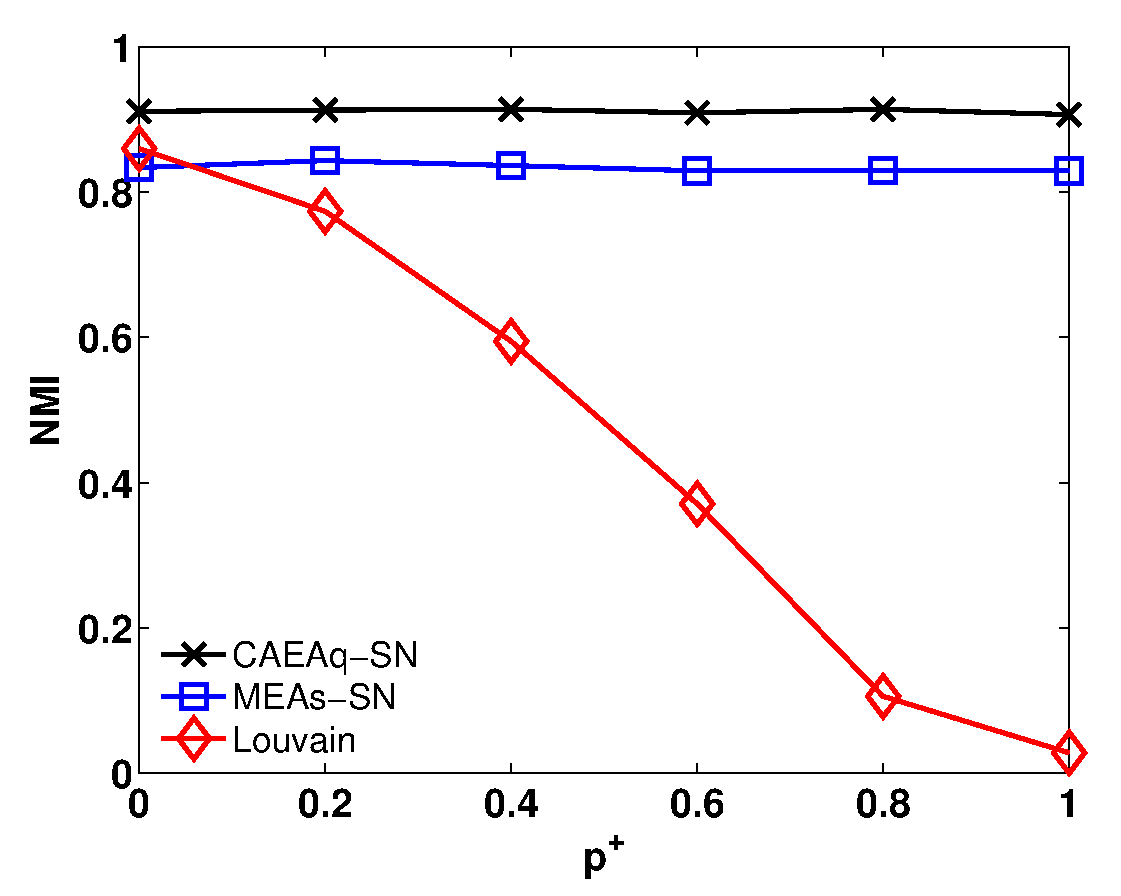
\includegraphics[width = 0.47\linewidth]{./Figure/dynamicmore/nmi5000mu03pn04.eps}	
 	}
 	\caption{Further comparison on SN5000. (a)$\mu=0.1,P^-=0.0$. (b)$\mu=0.1,P^-=0.2$. (c)$\mu=0.3,P^-=0.2$. (d)$\mu=0.3,P^-=0.4$.}
    \label{fig:SN5000Comparison}
\end{figure}

\begin{figure}[!htbp]
 	\centering
 	\subfloat[]{
 		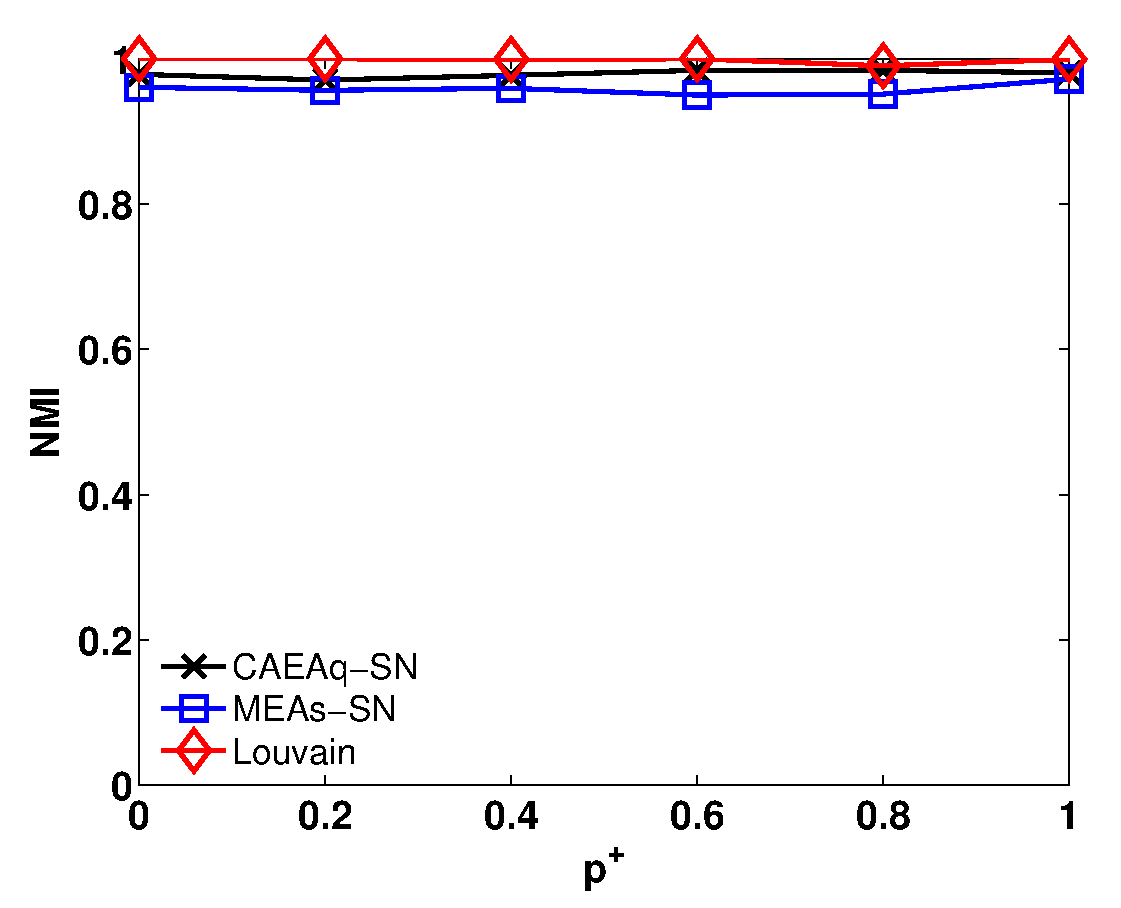
\includegraphics[width = 0.47\linewidth]{./Figure/dynamicmore/nmi10000mu01pn00.eps}	
 	}
 	\subfloat[]{
 		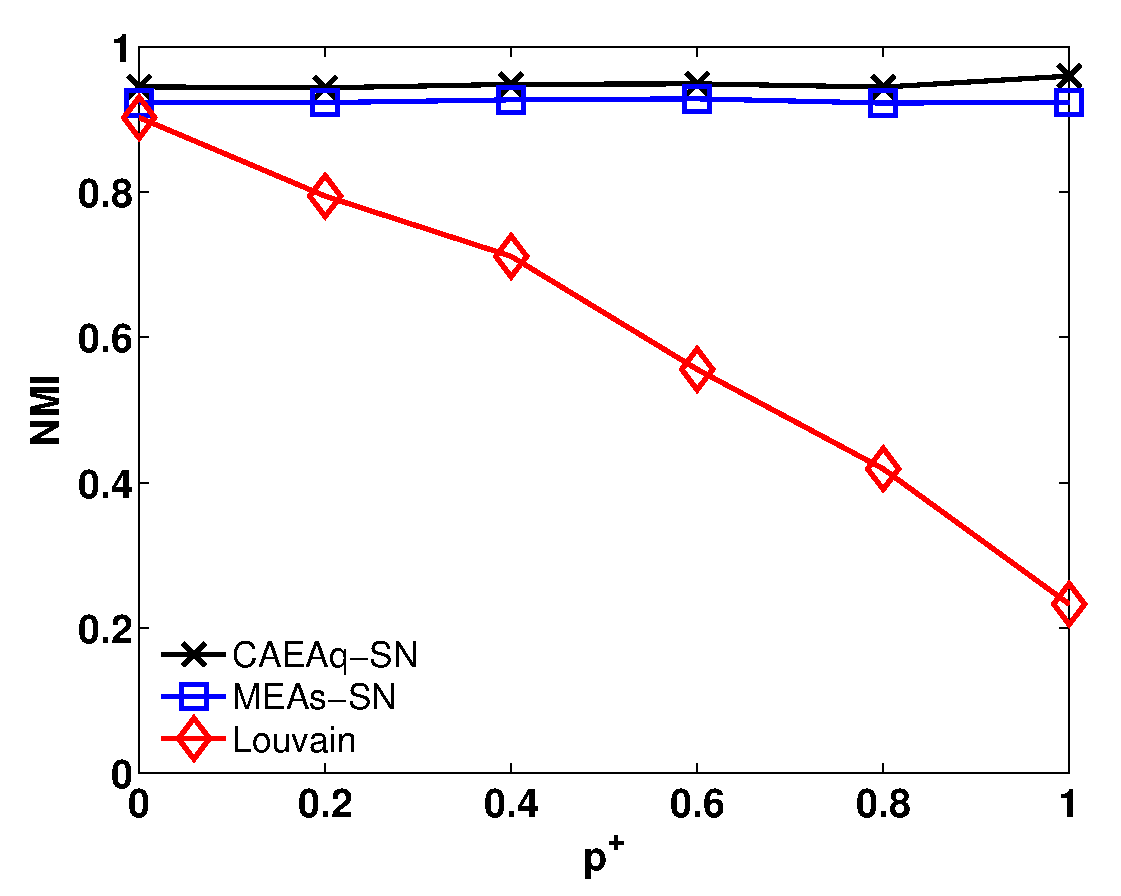
\includegraphics[width = 0.47\linewidth]{./Figure/dynamicmore/nmi10000mu01pn02.eps}	
 	}\\
 	\subfloat[]{
 		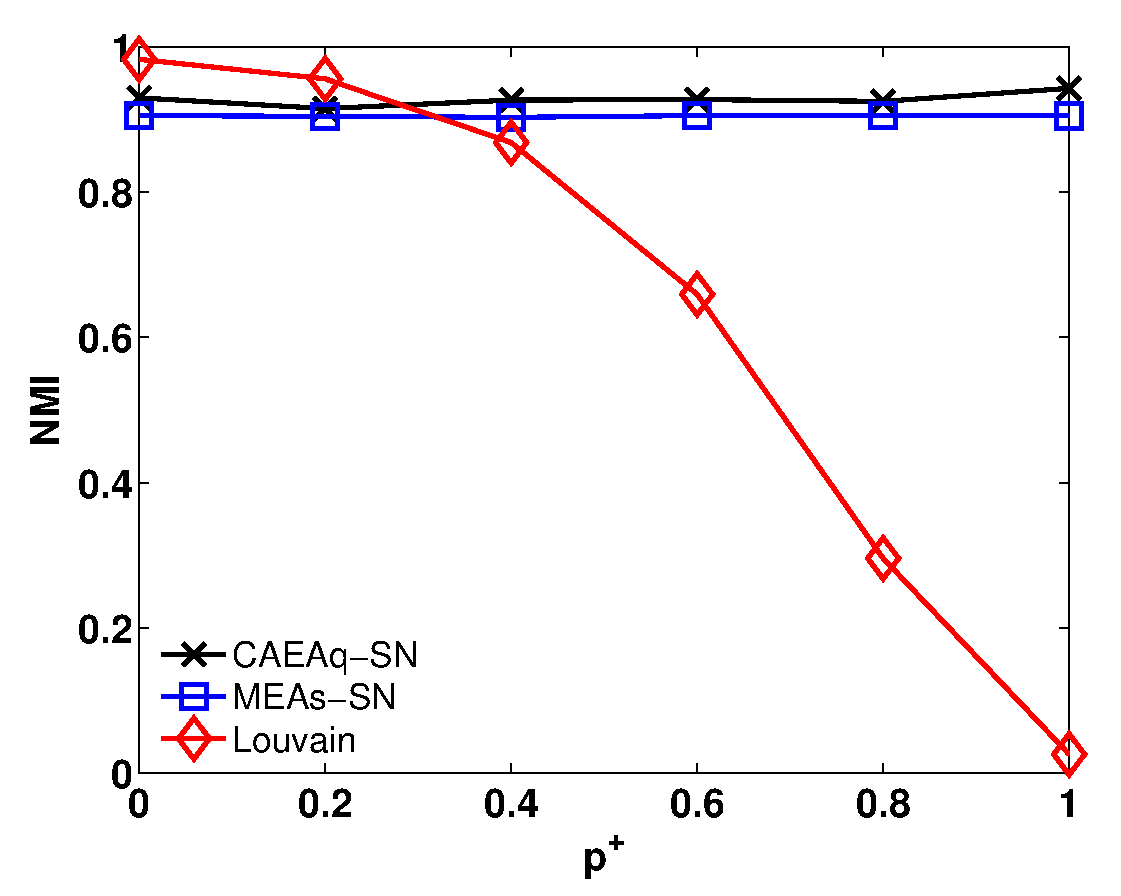
\includegraphics[width = 0.47\linewidth]{./Figure/dynamicmore/nmi10000mu03pn02.eps}	
  	}
    \subfloat[]{
 		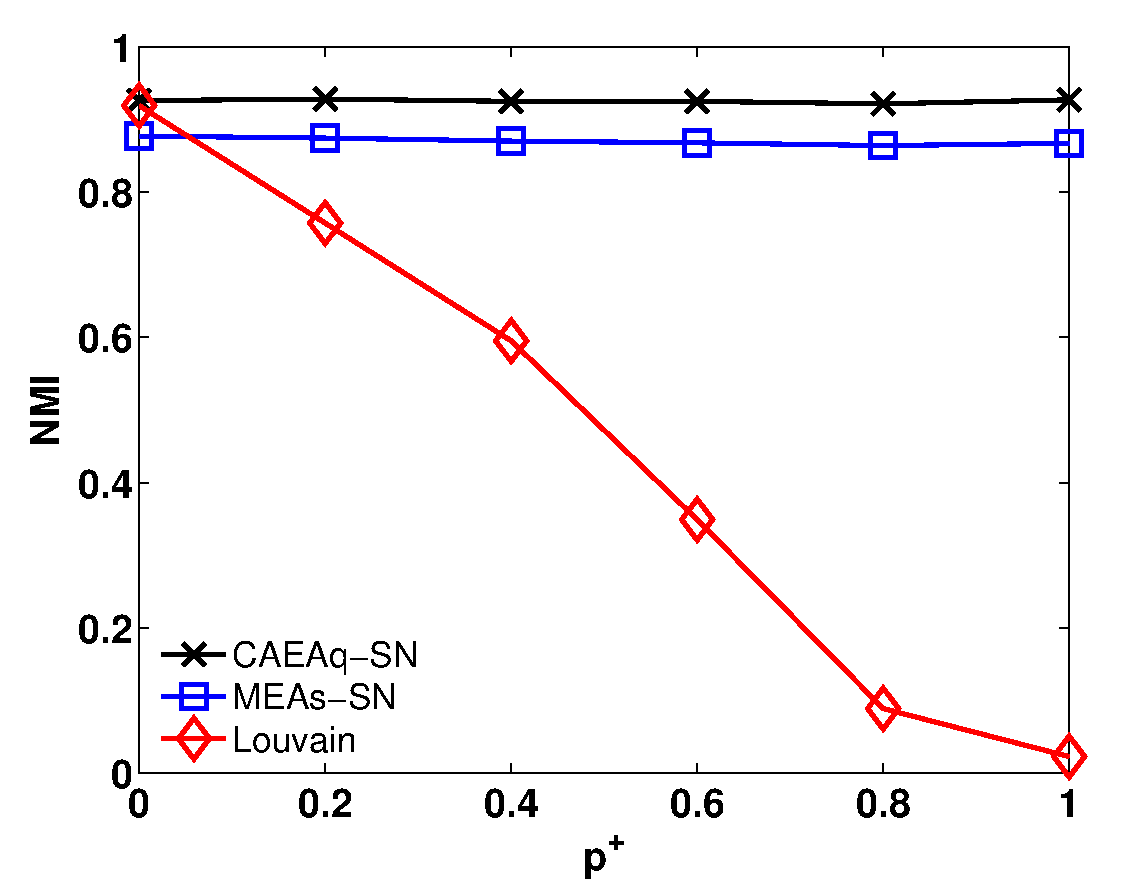
\includegraphics[width = 0.47\linewidth]{./Figure/dynamicmore/nmi10000mu03pn04.eps}	
 	}
 	\caption{Further comparison on SN10000. (a)$\mu=0.1,P^-=0.0$. (b)$\mu=0.1,P^-=0.2$. (c)$\mu=0.3,P^-=0.2$. (d)$\mu=0.3,P^-=0.4$.}
    \label{fig:SN10000Comparison}
\end{figure}

The results also indicate that two algorithms are sensitive to $P^-$ and insensitive to $P^+$. With the increase of $P^-$, the noise level increases, which destroys the network community structure and increases the ambiguous of the community structure significantly. For instance, when $P^- \geq 0.4$, all the values of Q are smaller than 0.3. Relatively speaking, comparison of performance is more meaningful when $P^-$ takes $\{0,0.2 \}$. Similarly, most of the Q are smaller than 0.3 when $\mu \geq 0.5$. Therefore, the separate comparisons of performance is discussed when $\mu$ takes $\{0.1,0.3\}$ and $P^-$ takes $\{0,0.2\}$.

Figs. \ref{fig:SN5000Comparison} and \ref{fig:SN10000Comparison} show further comparison on 5000 and 10000 nodes of synthetic SNs  between CAEAh-SN, MEAs-SN and Louvain method. Calculations indicate that NMI of the first two algorithms in SRN5000 is more stable than it in SN100 when $P^-$ and $\mu$ are fixed. CAEAh-SN obtains obviously higher Q than MEAs-SN for all the dynamic synthetic SNs.

In Fig. \ref{fig:SN100Comparisonmore}, the performance of CAEAh-SN is not only batter than MEAs-SN, but also more stable than MEAs-SN. Two algorithms are incomparable with each other only when $\mu=0.1, P^-=0.2$, and $P^+=0.8$.


In Fig. \ref{fig:SN500Comparisonmore}, the performance of CAEAh-SN outperforms MEAs-SN in the mass. It is worth noting that MEAs-SN fails to obtain partitions of which Q are not 0.

As a whole, the proposed CAEAh-SN obtains higher Q than MEAs-SN in terms of the solution quality, which implies the detected communities from SNs have better partitions by CAEAh-SN. Furthermore, CAEAh-SN is computationally much more efficient than MEAs-SN and shows a strong anti-perturbation performance and faster convergence rate.

\subsubsection{Comparison between CAEAh-SN and Louvain Method}
Besides comparing modularity of different algorithms, we also obtained NMI of detected communities from large-scale synthetic SNs. NMI measures the difference between the partition of community obtained by algorithms and the real partition. In this experiment, a series of large-scale SNs containing 10000 vertices are used to compare the performance of CAEAh-SN and Louvain Method, which can be formulated as the follow:
\begin{equation} \label{equ:large SNs}
SN(10000,5,15,2,1,40,100,0.1,P^+,P^-).
\end{equation}

Then, $P^+$ increases from 0.0 to 1.0 in the step of 0.2, and $P^-$ increases from 0.0 to 0.4 in the step of 0.2. For each network, two algorithms are executed 10 times. The average NMI values over these 10 runs are reported in Fig. \ref{fig:SN10000Comparisonmore}.

Fig. \ref{fig:SN10000Comparisonmore} clearly shows both CAEAh-SN and Louvain Method are almost always higher than 0.9 and close to 1.0 when $P^-=0.0$ and $P^+$ increases from 0.0 to 1.0. However, Louvain Method is so sensitive to the increase of $P^+$ that it's solutions drop dramatically when $P^-=0.2$ and $P^-=0.4$. For example, the NMI of CAEAh-SN is still higher than 0.8 but the NMI of Louvain Method drop to 0.2 when $P^-=0.2$ and $P^+=1.0$. More importantly, when $P^-=0.2$ and $P^-=0.4$, the NMI of CAEAh-SN is better than that of Louvain method when $P^+$ increases from 0.0 to 1.0 in most cases. The obtained results show that CAEAh-SN has stronger robustness to the SNs with high noises


\section{Conclusion}\label{section:conclusion}
In this paper, CAEAh-SN is proposed to extend the decomposition-based CAEA for CD from SNs. In CAEAh-SN, the modularity Q is partitioned into $Q^+$ and $Q^-$. The problem behaves like a bi-objective problem where $Q^+$ represents the development of the network towards the formation of the community, and $Q^-$ destroys the formation of the community. Moreover, an improved version of AreaTour algorithm which has been applied in CAEA algorithm, called QmodulTour, uses the modularity Q to select individuals. QmodulTour avoids the deviation of the evolution vector and improves computational efficiencies. The experimental results indicate that CAEAh-SN offers significantly higher Q than MEAs-SN in benchmark signed networks, synthetic networks with the general parameters, and synthetic networks with the dynamic parameters. Furthermore, our future research will focus on the large scale of SNs.



% trigger a \newpage just before the given reference
% number - used to balance the columns on the last page
% adjust value as needed - may need to be readjusted if
% the document is modified later
%\IEEEtriggeratref{8}
% The "triggered" command can be changed if desired:
%\IEEEtriggercmd{\enlargethispage{-5in}}

% references section

% can use a bibliography generated by BibTeX as a .bbl file
% BibTeX documentation can be easily obtained at:
% http://mirror.ctan.org/biblio/bibtex/contrib/doc/
% The IEEEtran BibTeX style support page is at:
% http://www.michaelshell.org/tex/ieeetran/bibtex/
\bibliographystyle{bib/IEEEtran}
% argument is your BibTeX string definitions and bibliography database(s)
\bibliography{bib/CAEAqSN}
%
% <OR> manually copy in the resultant .bbl file
% set second argument of \begin to the number of references
% (used to reserve space for the reference number labels box)
%\begin{thebibliography}{1}

%\bibitem{IEEEhowto:kopka}
%H.~Kopka and P.~W. Daly, \emph{A Guide to \LaTeX}, 3rd~ed.\hskip 1em plus
%  0.5em minus 0.4em\relax Harlow, England: Addison-Wesley, 1999.
%
%\end{thebibliography}


	\begin{IEEEbiography}[{
\includegraphics[width=1in,height=1.25in,clip,keepaspectratio]{photo/wying.eps}}]{Weiqin Ying}
		received the B.Sc. degree in computer science and technology from
		Chongqing University, Chongqing, China, in 2001, the M.Sc. degree
		and the Ph.D. degree in computer software and theory from Wuhan
		University, Wuhan, China, in 2005 and 2009, respectively.

        He is currently an Associate Professor with the School of Software
		Engineering, South China University of Technology, Guangzhou, China.
		His current research interests include evolutionary and genetic
		algorithms, multi-objective optimization and decision, distributed computing, deep learning, and relevant real-world
		applications.
		
	\end{IEEEbiography}

\begin{IEEEbiography}[{
\includegraphics[width=1in,height=1.25in,clip,keepaspectratio]{photo/pengfeichao.eps}}]{Pengfei Chao}
		received the B.Sc. degree in automation  from
		Henan Polytechnic University, Jiaozuo, China, in 2016, and is currently
        pursuing his M.Eng. degree in software engineering from the School of Software Engineering,
        South China University of Technology, Guangzhou, China.

        His current research interests include evolutionary algorithms and their
        applications on real-world problems.	
	\end{IEEEbiography}	
	
\begin{IEEEbiography}[{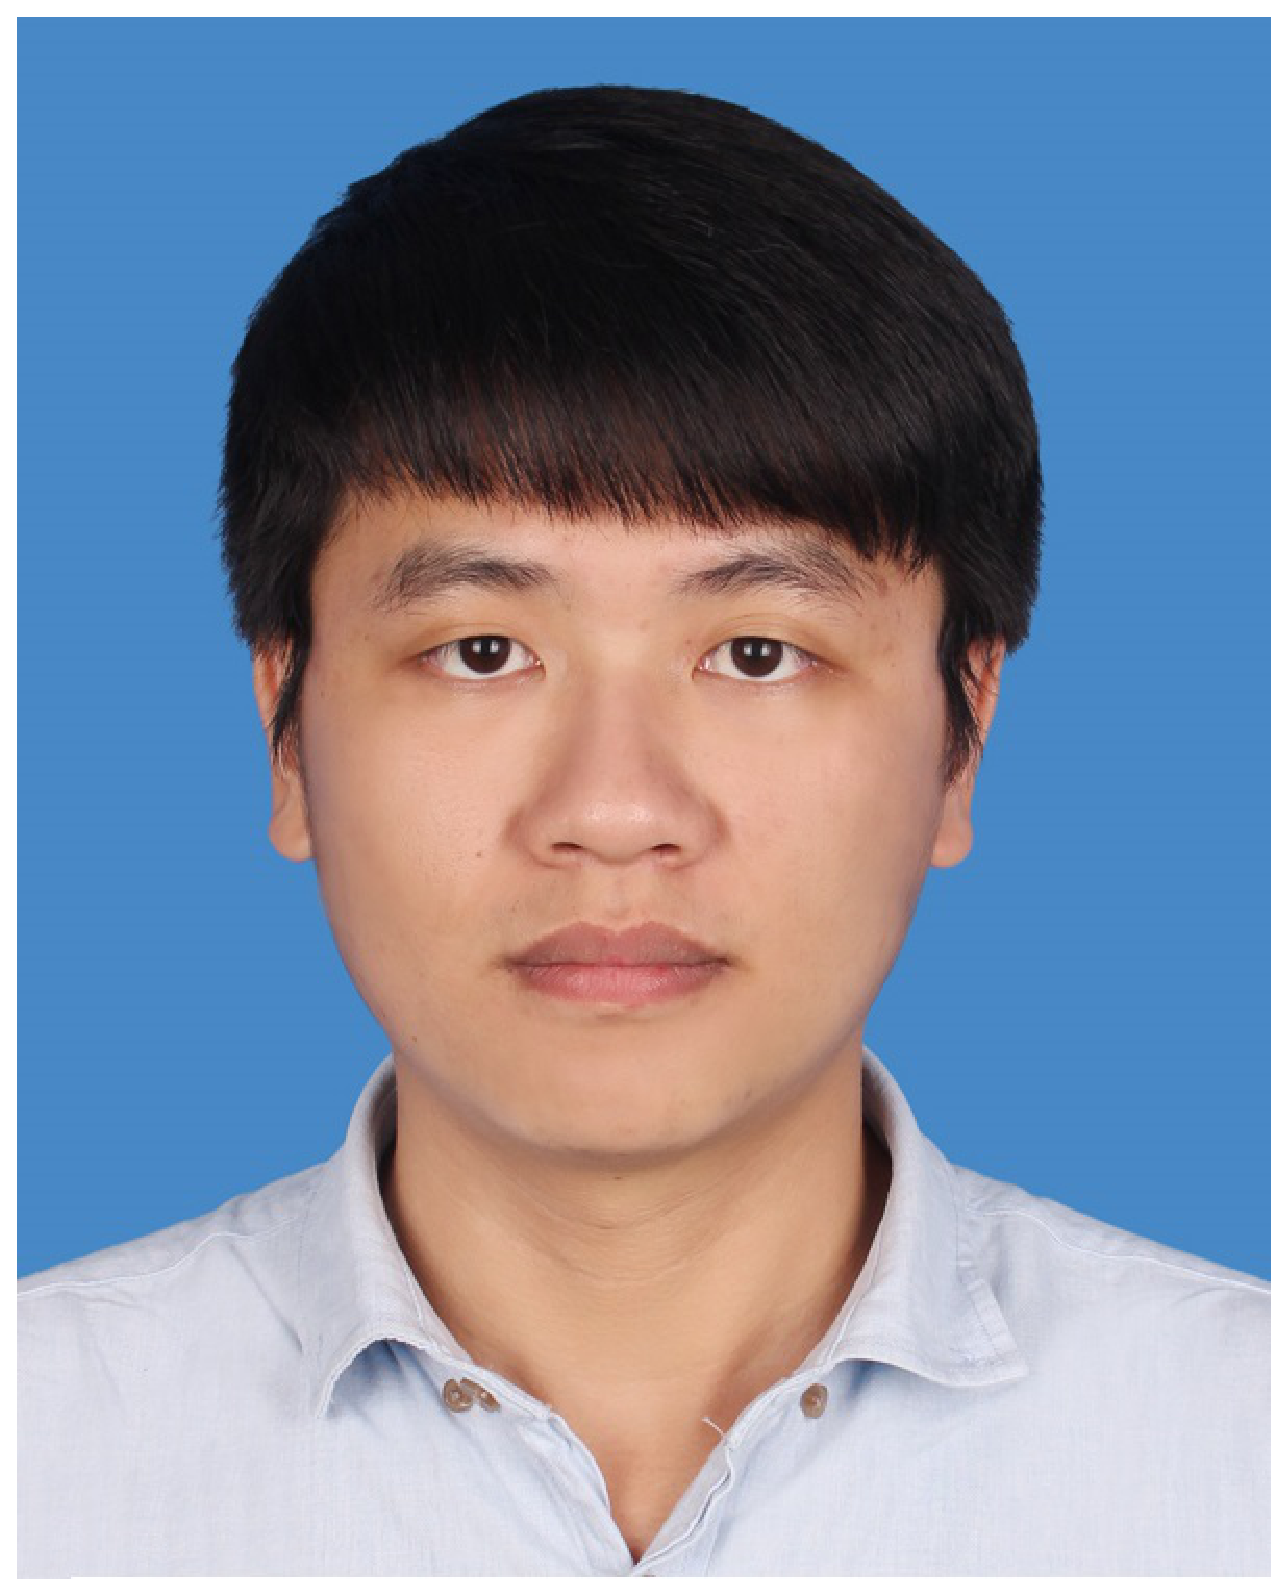
\includegraphics[width=1in,height=1.25in,clip,keepaspectratio]{photo/yxie.eps}}]{Yuehong Xie}
		received the B.Sc. degree and the M.Eng. degree in software engineering
        from South China University of Technology, Guangzhou, China, in 2014 and
        2017, respectively.
		
		His current research interests include multi-objective optimization, many-objective optimization, evolutionary algorithms
		and constrained handling techniques.
	\end{IEEEbiography}
	
\begin{IEEEbiography}[{
\includegraphics[width=1in,height=1.25in,clip,keepaspectratio]{photo/zhenyuwang.eps}}]{Zhenyu Wang}
        received the B.Sc. degree in computer science and technology from
		Xiamen University, Xiamen, China, in 1987, the M.Sc. degree in computer application
		and the Ph.D. degree in computer architecture from Harbin Institute of Technology, Harbin, China, in 1990 and 1993, respectively.		

        He is currently a Professor and the dean with the School of Software Engineering, South China University of Technology, Guangzhou, China.		
		His current research interests include distributed
        computing, cloud computing, big data technologies, service-oriented architecture, large-scale application design and development, and multi-objective optimization.
	\end{IEEEbiography}

	\begin{IEEEbiography}[{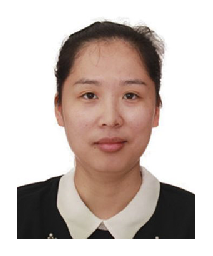
\includegraphics[width=1in,height=1.25in,clip,keepaspectratio]{photo/yuwu.eps}}]{Yu Wu}
		received the B.Sc. degree in computer science and technology from
		Chongqing University, Chongqing, China, in 2001, the M.Sc. degree
		and the Ph.D. degree in computer software and theory from Wuhan
		University, Wuhan, China, in 2005 and 2009, respectively.

        He is currently an Associate Professor with the School of Software
		Engineering, South China University of Technology, Guangzhou, China.
		His current research interests include evolutionary and genetic
		algorithms, multi-objective optimization and decision, distributed computing, deep learning, and relevant real-world
		applications.
		
	\end{IEEEbiography}

% that's all folks


\end{document}


